\documentclass[10pt]{beamer}

% Beamer style
%\usetheme[secheader]{Madrid}
\usetheme{CambridgeUS}
\usecolortheme[rgb={0.65,0.15,0.25}]{structure}
%\usefonttheme[onlymath]{serif}
\beamertemplatenavigationsymbolsempty
%\AtBeginSubsection

% Packages
%\usepackage[french]{babel}
\usepackage[latin1]{inputenc}
\usepackage{color}
\usepackage{xspace}
%\usepackage{dsfont, stmaryrd}
\usepackage{amsmath, amsfonts, amssymb}
\usepackage{url}
% \usepackage{/home/robin/LATEX/Biblio/astats}
%\usepackage[all]{xy}
\usepackage{graphicx}

% Commands
\definecolor{darkred}{rgb}{0.65,0.15,0.25}
\newcommand{\emphase}[1]{\textcolor{darkred}{#1}}
%\newcommand{\emphase}[1]{{#1}}
\newcommand{\paragraph}[1]{\textcolor{darkred}{#1}}
\newcommand{\refer}[1]{{{\textcolor{blue}{{\cite{#1}}}}}}
\newcommand{\Refer}[1]{{{\textcolor{blue}{{\sl #1}}}}}
% \newcommand{\newblock}{}

% Symbols
% \newcommand{\Abf}{{\bf A}}
\newcommand{\Beta}{\text{B}}
\newcommand{\Bcal}{\mathcal{B}}
\newcommand{\BIC}{\text{BIC}\xspace}
\newcommand{\Ccal}{\mathcal{C}}
\newcommand{\dd}{\text{~d}}
% \newcommand{\dbf}{{\bf d}}
\newcommand{\Dcal}{\mathcal{D}}
\newcommand{\Esp}{\mathbb{E}}
% \newcommand{\Ebf}{{\bf E}}
\newcommand{\Ecal}{\mathcal{E}}
\newcommand{\Gcal}{\mathcal{G}}
\newcommand{\Gam}{\mathcal{G}\text{am}}
\newcommand{\Ibb}{\mathbb{I}}
% \newcommand{\Ibf}{{\bf I}}
\newcommand{\ICL}{\text{ICL}\xspace}
\newcommand{\Cov}{\mathbb{C}\text{ov}}
\newcommand{\Corr}{\mathbb{C}\text{orr}}
\newcommand{\Var}{\mathbb{V}}
\newcommand{\Vsf}{\mathsf{V}}
\newcommand{\pen}{\text{pen}}
\newcommand{\Fcal}{\mathcal{F}}
% \newcommand{\Hbf}{{\bf H}}
\newcommand{\Hcal}{\mathcal{H}}
\newcommand{\Jcal}{\mathcal{J}}
% \newcommand{\Kbf}{{\bf K}}
\newcommand{\Lcal}{\mathcal{L}}
\newcommand{\Mcal}{\mathcal{M}}
% \newcommand{\mbf}{{\bf m}}
% \newcommand{\mum}{\mu(\mbf)}
\newcommand{\Ncal}{\mathcal{N}}
% \newcommand{\Nbf}{{\bf N}}
% \newcommand{\Nm}{N(\mbf)}
\newcommand{\Ocal}{\mathcal{O}}
% \newcommand{\Obf}{{\bf 0}}
\newcommand{\Omegas}{\underset{s}{\Omega}}
% \newcommand{\Pbf}{{\bf P}}
\newcommand{\Pcal}{\mathcal{P}}
\newcommand{\Qcal}{\mathcal{Q}}
\newcommand{\Rbb}{\mathbb{R}}
\newcommand{\Rcal}{\mathcal{R}}
% \newcommand{\sbf}{{\bf s}}
% \newcommand{\Sbf}{{\bf S}}
\newcommand{\Scal}{\mathcal{S}}
\newcommand{\Ucal}{\mathcal{U}}
\newcommand{\Vcal}{\mathcal{V}}
\newcommand{\BP}{\text{BP}}
\newcommand{\EM}{\text{EM}}
\newcommand{\VEM}{\text{VEM}}
\newcommand{\VBEM}{\text{VBEM}}
\newcommand{\cst}{\text{cst}}
\newcommand{\obs}{\text{obs}}
\newcommand{\ra}{\emphase{\mathversion{bold}{$\rightarrow$}~}}
\newcommand{\QZ}{Q_{Z}}
\newcommand{\Qt}{Q_{\theta}}
%\newcommand{\transp}{\text{{\tiny $\top$}}}
\newcommand{\transp}{\text{{\tiny \mathversion{bold}{$\top$}}}}

\newcommand{\beginbackup}{
   \newcounter{framenumbervorappendix}
   \setcounter{framenumbervorappendix}{\value{framenumber}}
}
\newcommand{\backupend}{
   \addtocounter{framenumbervorappendix}{-\value{framenumber}}
   \addtocounter{framenumber}{\value{framenumbervorappendix}} 
}


% Directory
\newcommand{\figmixt}{/home/robin/ENSEIGN/COURS/MELANGE}
\newcommand{\figbma}{/home/robin/RECHERCHE/RUPTURES/MELANGE/Exemples/Grippe}
\newcommand{\fignet}{/home/robin/RECHERCHE/RESEAUX/EXPOSES/FIGURES}
\newcommand{\figeco}{/home/robin/RECHERCHE/ECOLOGIE/EXPOSES/FIGURES}
%\newcommand{\figmotif}{/home/robin/RECHERCHE/RESEAUX/Motifs/FIGURES}


%====================================================================
\title[Variational inference for $W$-graphs]{{Averaging Stochastic Block Models to estimate the graphon function}}
  
% Bayesian model averaging of stochastic block models to estimate the graphon function 
% Averaging Stochastic Block Models to estimate the graphon function of a W-graph

\author{S. Robin}

\institute[INRA / AgroParisTech]{INRA / AgroParisTech \\
  \vspace{-.25\textheight}
  \begin{center}
  \begin{tabular}{ccccc}
    
\includegraphics[width=2.5cm]{../FIGURES/LogoINRA-Couleur} & 
    \hspace{.5cm} &
    
\includegraphics[width=3.75cm]{../FIGURES/logagroptechsolo} & 
    \hspace{.5cm} &
    
\includegraphics[width=2.5cm]{../FIGURES/logo-ssb}
    \\ 
  \end{tabular} 
  \end{center}
  \medskip
    {\normalsize joint work with P. Latouche} \\ ~\\
  }

\date[Dublin, July'14]{{\normalsize Working group on model-based clustering, July 2014, Dublin}}
%====================================================================

%====================================================================
%====================================================================
\begin{document}
%====================================================================
%====================================================================

%====================================================================
\frame{\titlepage}

%====================================================================
\section{Modeling network heterogeneity}
\frame{\frametitle{Modeling network heterogeneity}}
%====================================================================
\frame{\frametitle{Modeling network heterogeneity} 

  \paragraph{Latent variable models} allow to capture the underlying structure of a network.

  \bigskip \bigskip \pause
  \paragraph{General setting for binary graphs.} \refer{BJR07}: %\pause
  \begin{itemize}
   \item   {A latent (unobserved) variable $Z_i$} is associated with each node:
  $$
  \{Z_i\} \text{ iid } \sim \pi 
  $$
  \item 
  Edges {$X_{ij} = \Ibb\{i \sim j\}$ are independent conditionally} to the $Z_i$'s:
  $$
  \{X_{ij}\} \text{ independent } | \{Z_i\}: \Pr\{X_{ij} = 1\} = \gamma(Z_i, Z_j)
  $$
  \end{itemize}

  \bigskip 
  Includes latent position models \refer{HRH02,HRT07}, see \refer{MaR14} for a review.

  }

%====================================================================
\frame{\frametitle{Stochastic Block Model (SBM)}

  \begin{tabular}{cc}
    \hspace{-.5cm}
    \begin{tabular}{p{.5\textwidth}}
      \onslide+<1->{\paragraph{A mixture model for random graphs.}}
      \onslide+<2->{\begin{itemize}
        \item Consider $n$ nodes ($i = 1..n$); \\ ~ } 
        \onslide+<3->{
        \item $Z_i = $ unobserved label of node $i$:
          $$
          \{Z_i\} \text{ i.i.d. } \sim \Mcal(1; \pi)
          $$
          $\pi = (\pi_1, ... \pi_K)$; \\ ~ } 
        \onslide+<4->{
        \item Edge $X_{ij}$ depends on the labels:
          $\{X_{ij}\}$ independent given $\{Z_i\}$,
          $$
          (X_{ij}) \sim \Bcal(\gamma_{Z_i, Z_j})
          $$}
      \end{itemize}
    \end{tabular}
    & 
    \hspace{-.5cm}
    \begin{tabular}{p{.5\textwidth}}
      \vspace{1cm}
      \begin{overprint}
        \onslide<2>
        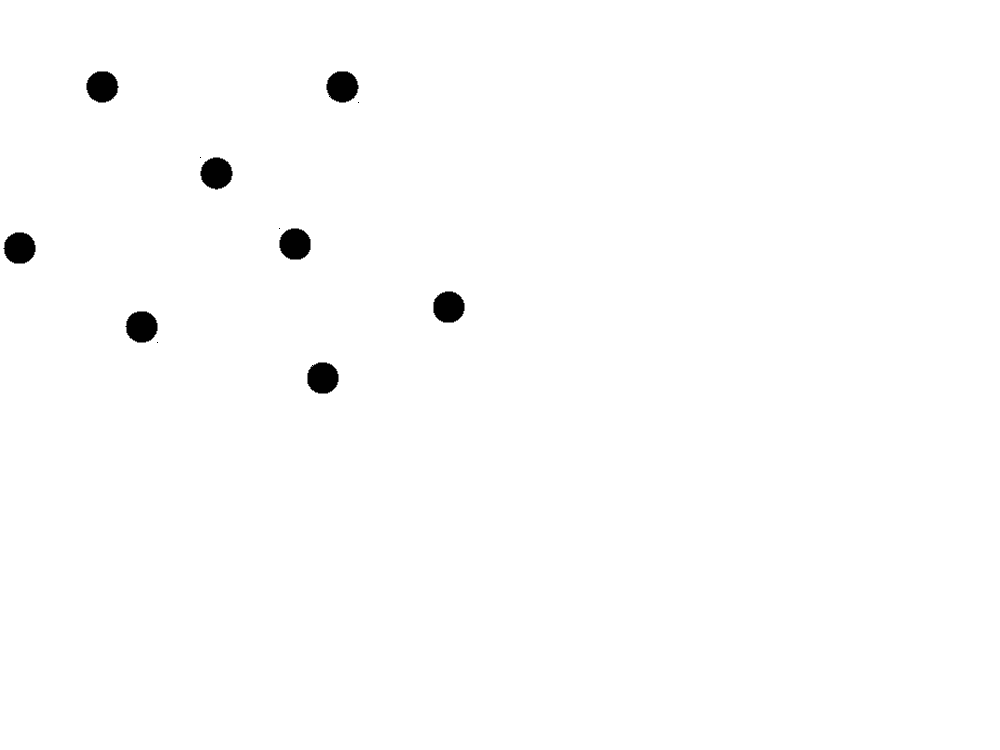
\includegraphics[width=.75\textwidth, clip=]{../FIGURES/FigSBM-Model-1}
        \onslide<3>
        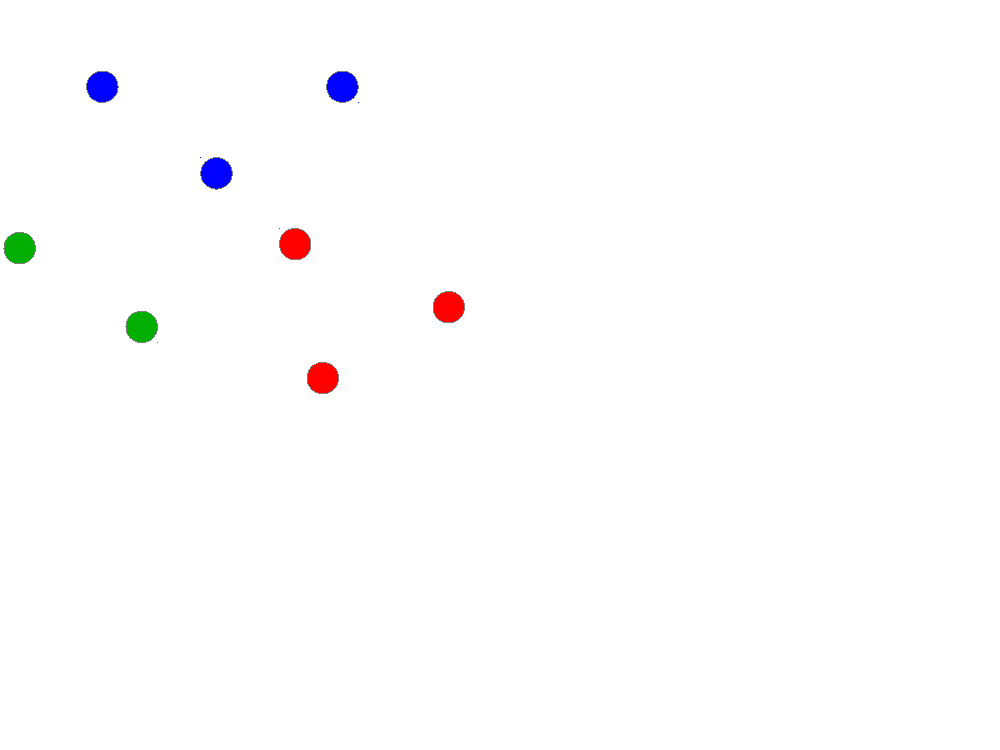
\includegraphics[width=.75\textwidth, clip=]{../FIGURES/FigSBM-Model-2}
        \onslide<4>
        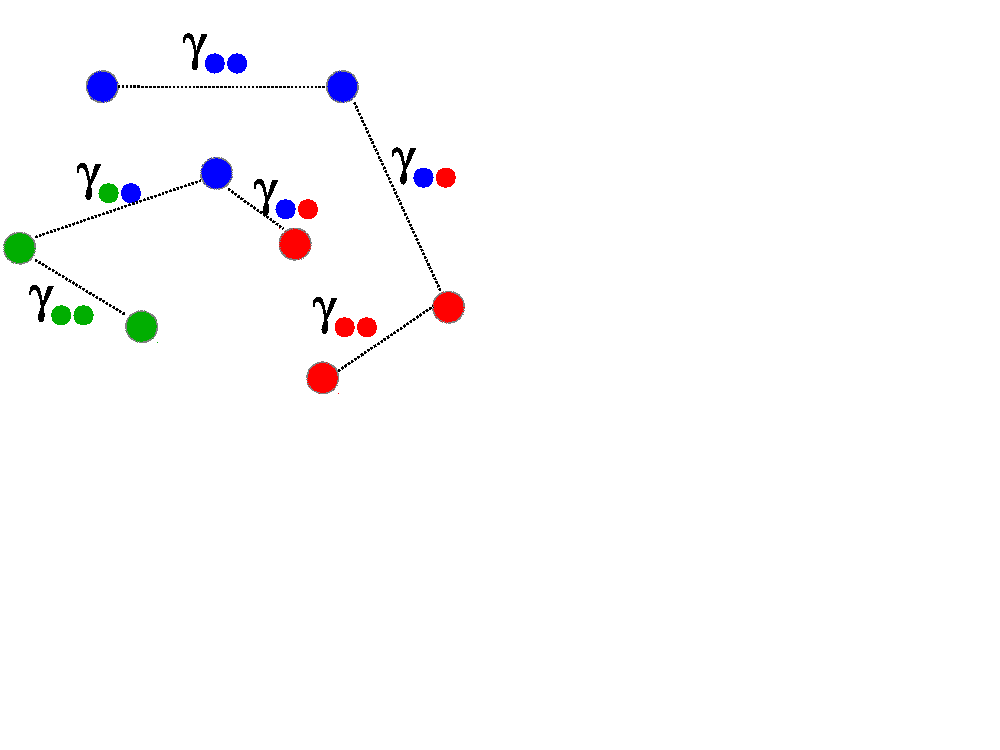
\includegraphics[width=.75\textwidth, clip=]{../FIGURES/FigSBM-Model-3}
        \onslide<5>
%         \includegraphics[width=.75\textwidth, clip=]{../FIGURES/FigSBM-Model-4}
%        \onslide<6>
        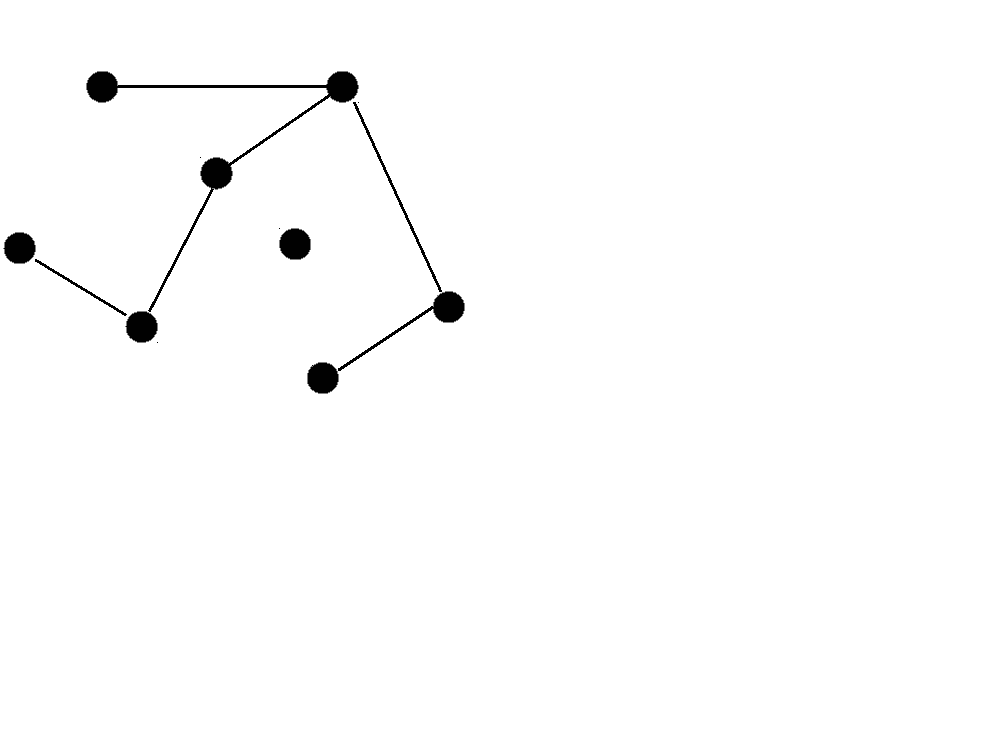
\includegraphics[width=.75\textwidth, clip=]{../FIGURES/FigSBM-Model-5}
      \end{overprint}
    \end{tabular}
  \end{tabular}
  }

%====================================================================
\frame{ \frametitle{$W$-graph model}

  \begin{tabular}{cc}
    \hspace{-.5cm}
    \begin{tabular}{p{.5\textwidth}}
	 Latent variables:
	 $$
	 (Z_i) \text{ iid } \sim \Ucal_{[0, 1]},
	 $$ ~\\
	 Graphon function $\gamma$:
	 $$
	 \gamma(z, z'): [0, 1]^2 \rightarrow [0, 1]
	 $$ ~\\    
	 Edges:
	 $$
	 \Pr\{X_{ij} = 1\} = \gamma(Z_i, Z_j)
	 $$    
	 \end{tabular}
    & 
    \hspace{-.1\textwidth}
    \begin{tabular}{p{.5\textwidth}}
	 Graphon function $\gamma(z, z')$ \\
      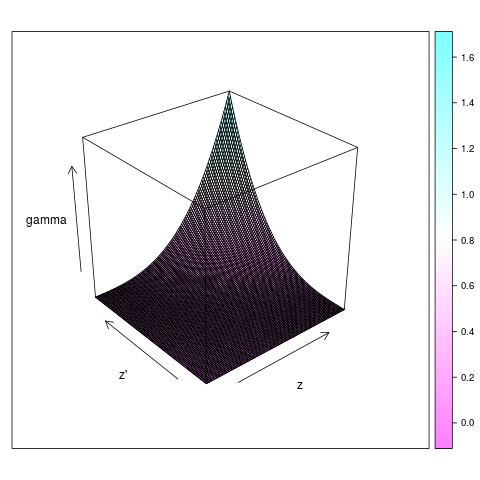
\includegraphics[width=.5\textwidth]{../FIGURES/FigCLADAG-W-graphon} \\
    \end{tabular}
  \end{tabular}
  
  \medskip
  \paragraph{Aim of this work:} provide an estimate of the graphon function.
%   Intensively studied in probability theory as a limit for dense graphs \refer{LoS06}.

 }

%====================================================================
\frame{\frametitle{Interpreting the graphon function}

  The graphon function provides a global picture of the network's topology.

  \bigskip \bigskip 
  \centerline{
  \begin{tabular}{ccc}
  'Scale free' & Community & Small world \\
  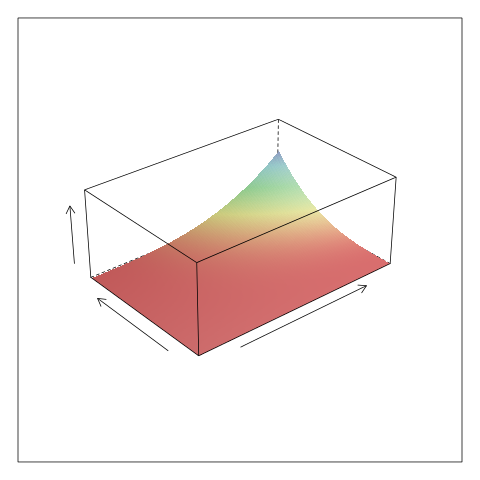
\includegraphics[width=.3\textwidth]{../FIGURES/EDD-ScaleFreeTrueGraphon} &
  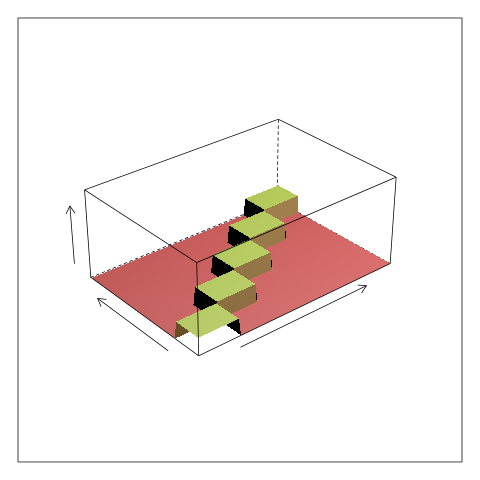
\includegraphics[width=.3\textwidth]{../FIGURES/CommunityTrueGraphon} &
  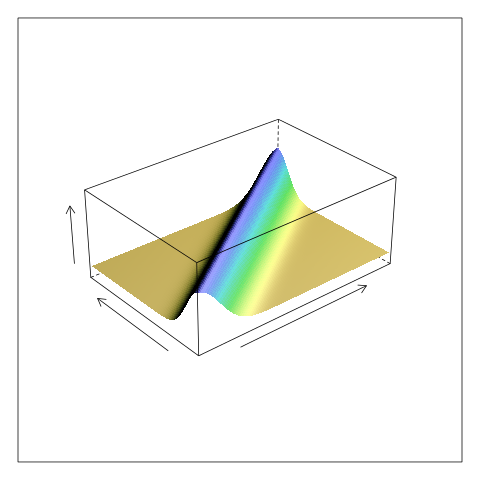
\includegraphics[width=.3\textwidth]{../FIGURES/SmallWorldTrueGraphon} 
  \end{tabular}
  }
  
}

%====================================================================
\section{Variational inference}
\frame{\frametitle{Variational inference}}
%====================================================================
\frame{\frametitle{Looking for conditional distributions}

  \begin{tabular}{cc}
    \hspace{-.5cm}
    \begin{tabular}{p{.5\textwidth}}
      \onslide+<1->{
        \paragraph{Maximum likelihood estimation} (e.g. EM) of $\theta = (\pi, \gamma)$ often requires the calculation of
        $$
        P_{\theta}(Z | X).
        $$
        ~\\~\\~\\
      }
    \end{tabular}
    & 
    \hspace{-.5cm}
    \begin{tabular}{p{.5\textwidth}}
            \begin{overprint}
        \onslide<2>
        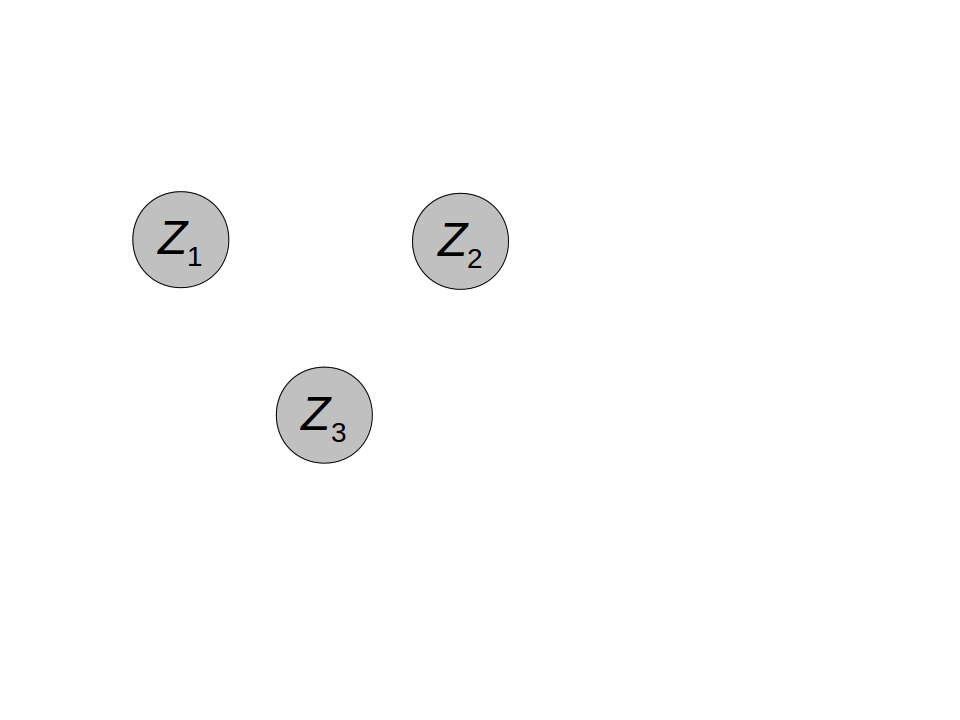
\includegraphics[width=.6\textwidth, clip=]{../FIGURES/FigSBM-Z}
        \onslide<3>
        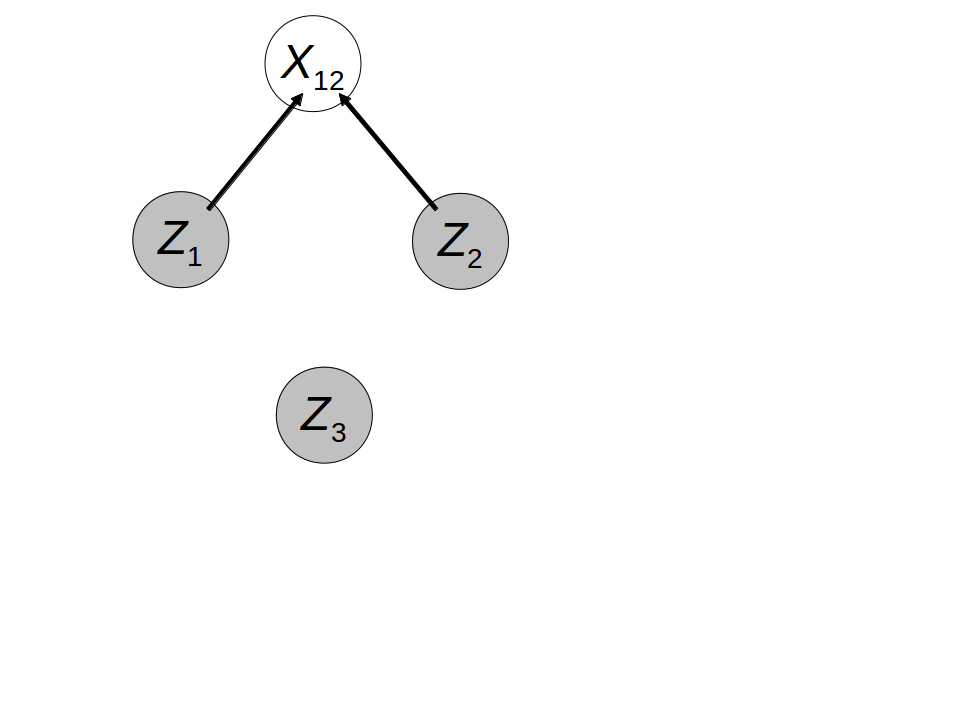
\includegraphics[width=.6\textwidth, clip=]{../FIGURES/FigSBM-Z-X12}
        \onslide<4>
        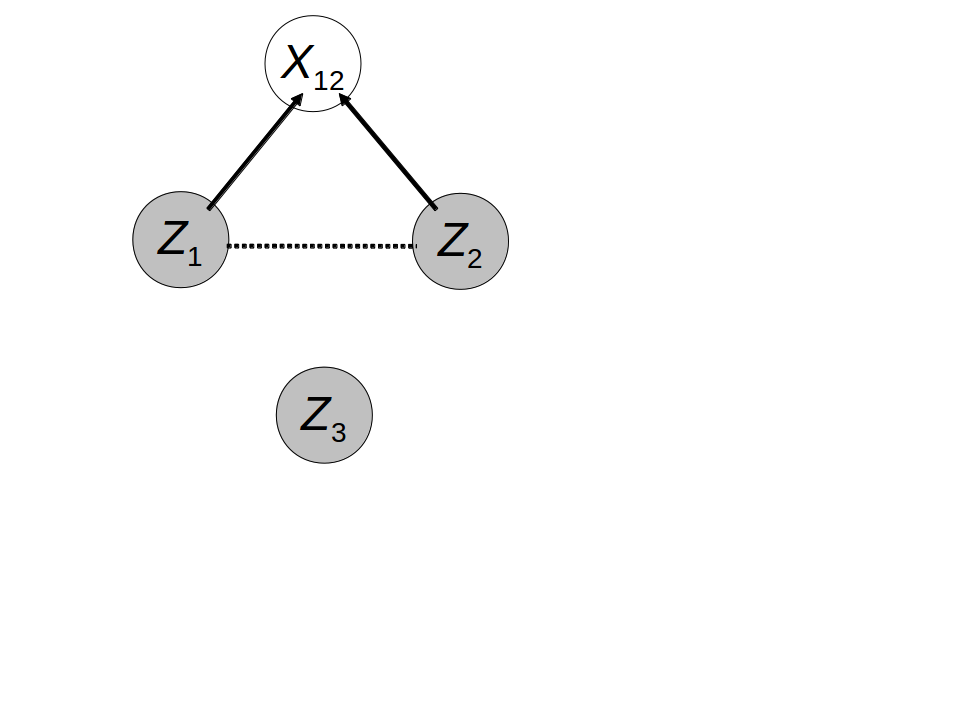
\includegraphics[width=.6\textwidth, clip=]{../FIGURES/FigSBM-Z-X12-Moral}
        \onslide<5>
        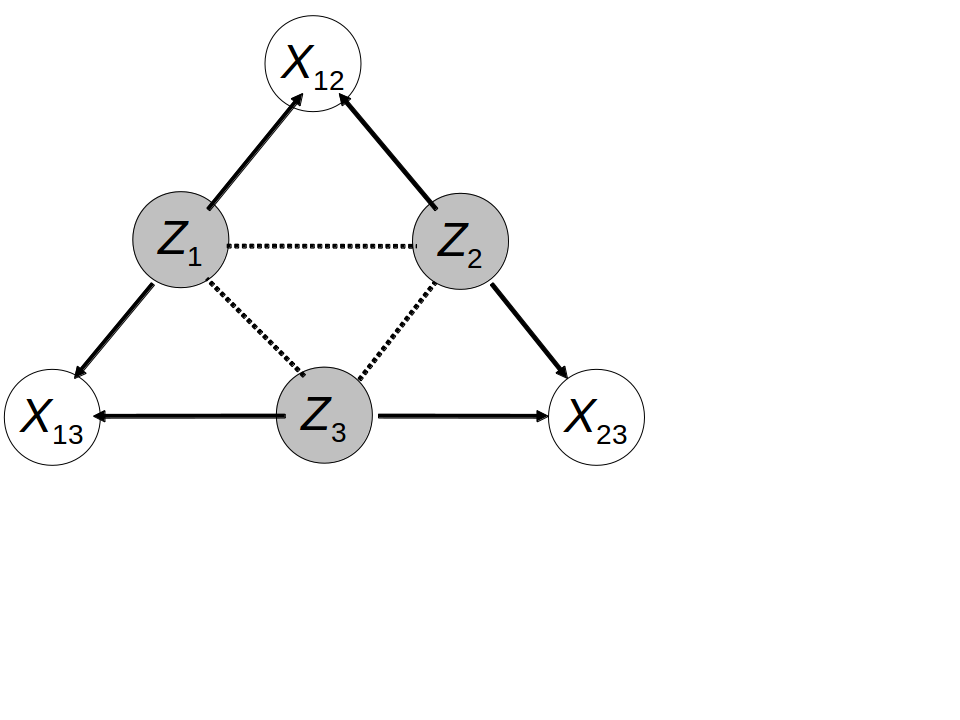
\includegraphics[width=.6\textwidth, clip=]{../FIGURES/FigSBM-Z-X-Moral}
        \onslide<6->
        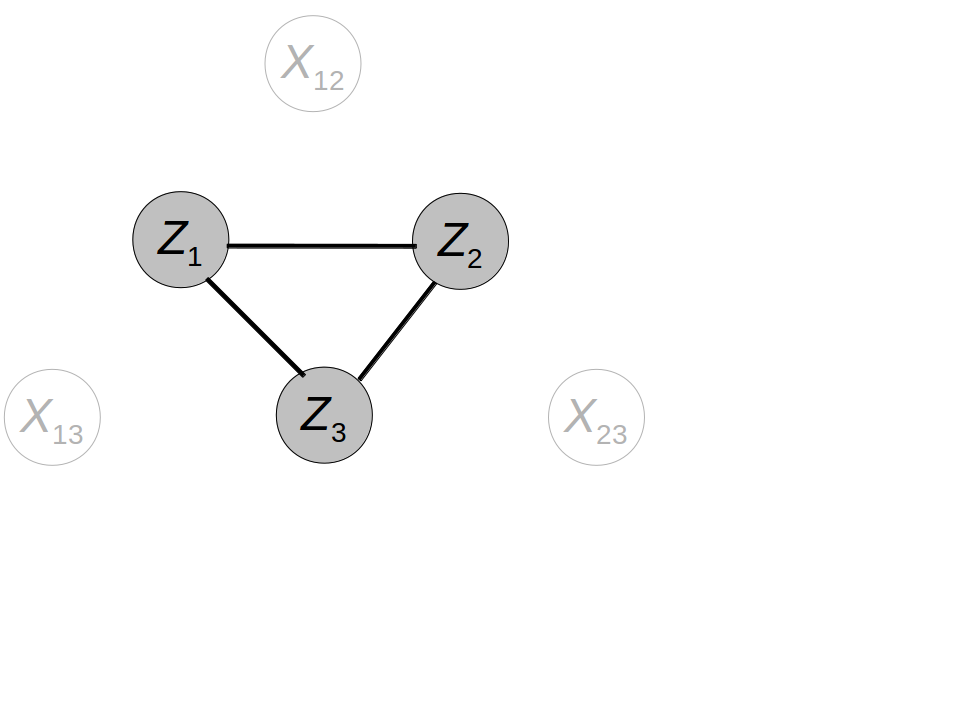
\includegraphics[width=.6\textwidth, clip=]{../FIGURES/FigSBM-ZcondX}
      \end{overprint}
    \end{tabular}
  \end{tabular}

  \onslide+<6->{
    \vspace{-.1\textheight}
    \paragraph{Conditional distribution.} The dependency graph of
    $Z$ given $X$ is a clique. \\
    \ra No factorization can be hoped (unlike for HMM). \\
    \ra $P_{\theta}(Z | X)$ can not be computed
    (efficiently). \\
%     \ra Variational techniques provide 
%     $$
%     Q(Z) \simeq P_{\theta}(Z | X).
%     $$
  }
}

%====================================================================
\frame{\frametitle{Looking for conditional distributions}
  
  \begin{tabular}{cc}
    \hspace{-.5cm}
    \begin{tabular}{p{.5\textwidth}}
      \paragraph{Bayesian inference.} We are now interested in 
      $$
      P(Z, \theta | X)
      $$
      \ra more intricate than $P_{\theta}(Z | X)$.
      \\~\\~\\~\\~\\
    \end{tabular}
    & 
    \hspace{-.5cm}
    \begin{tabular}{p{.5\textwidth}}
      \begin{overprint}
        \onslide<2>
        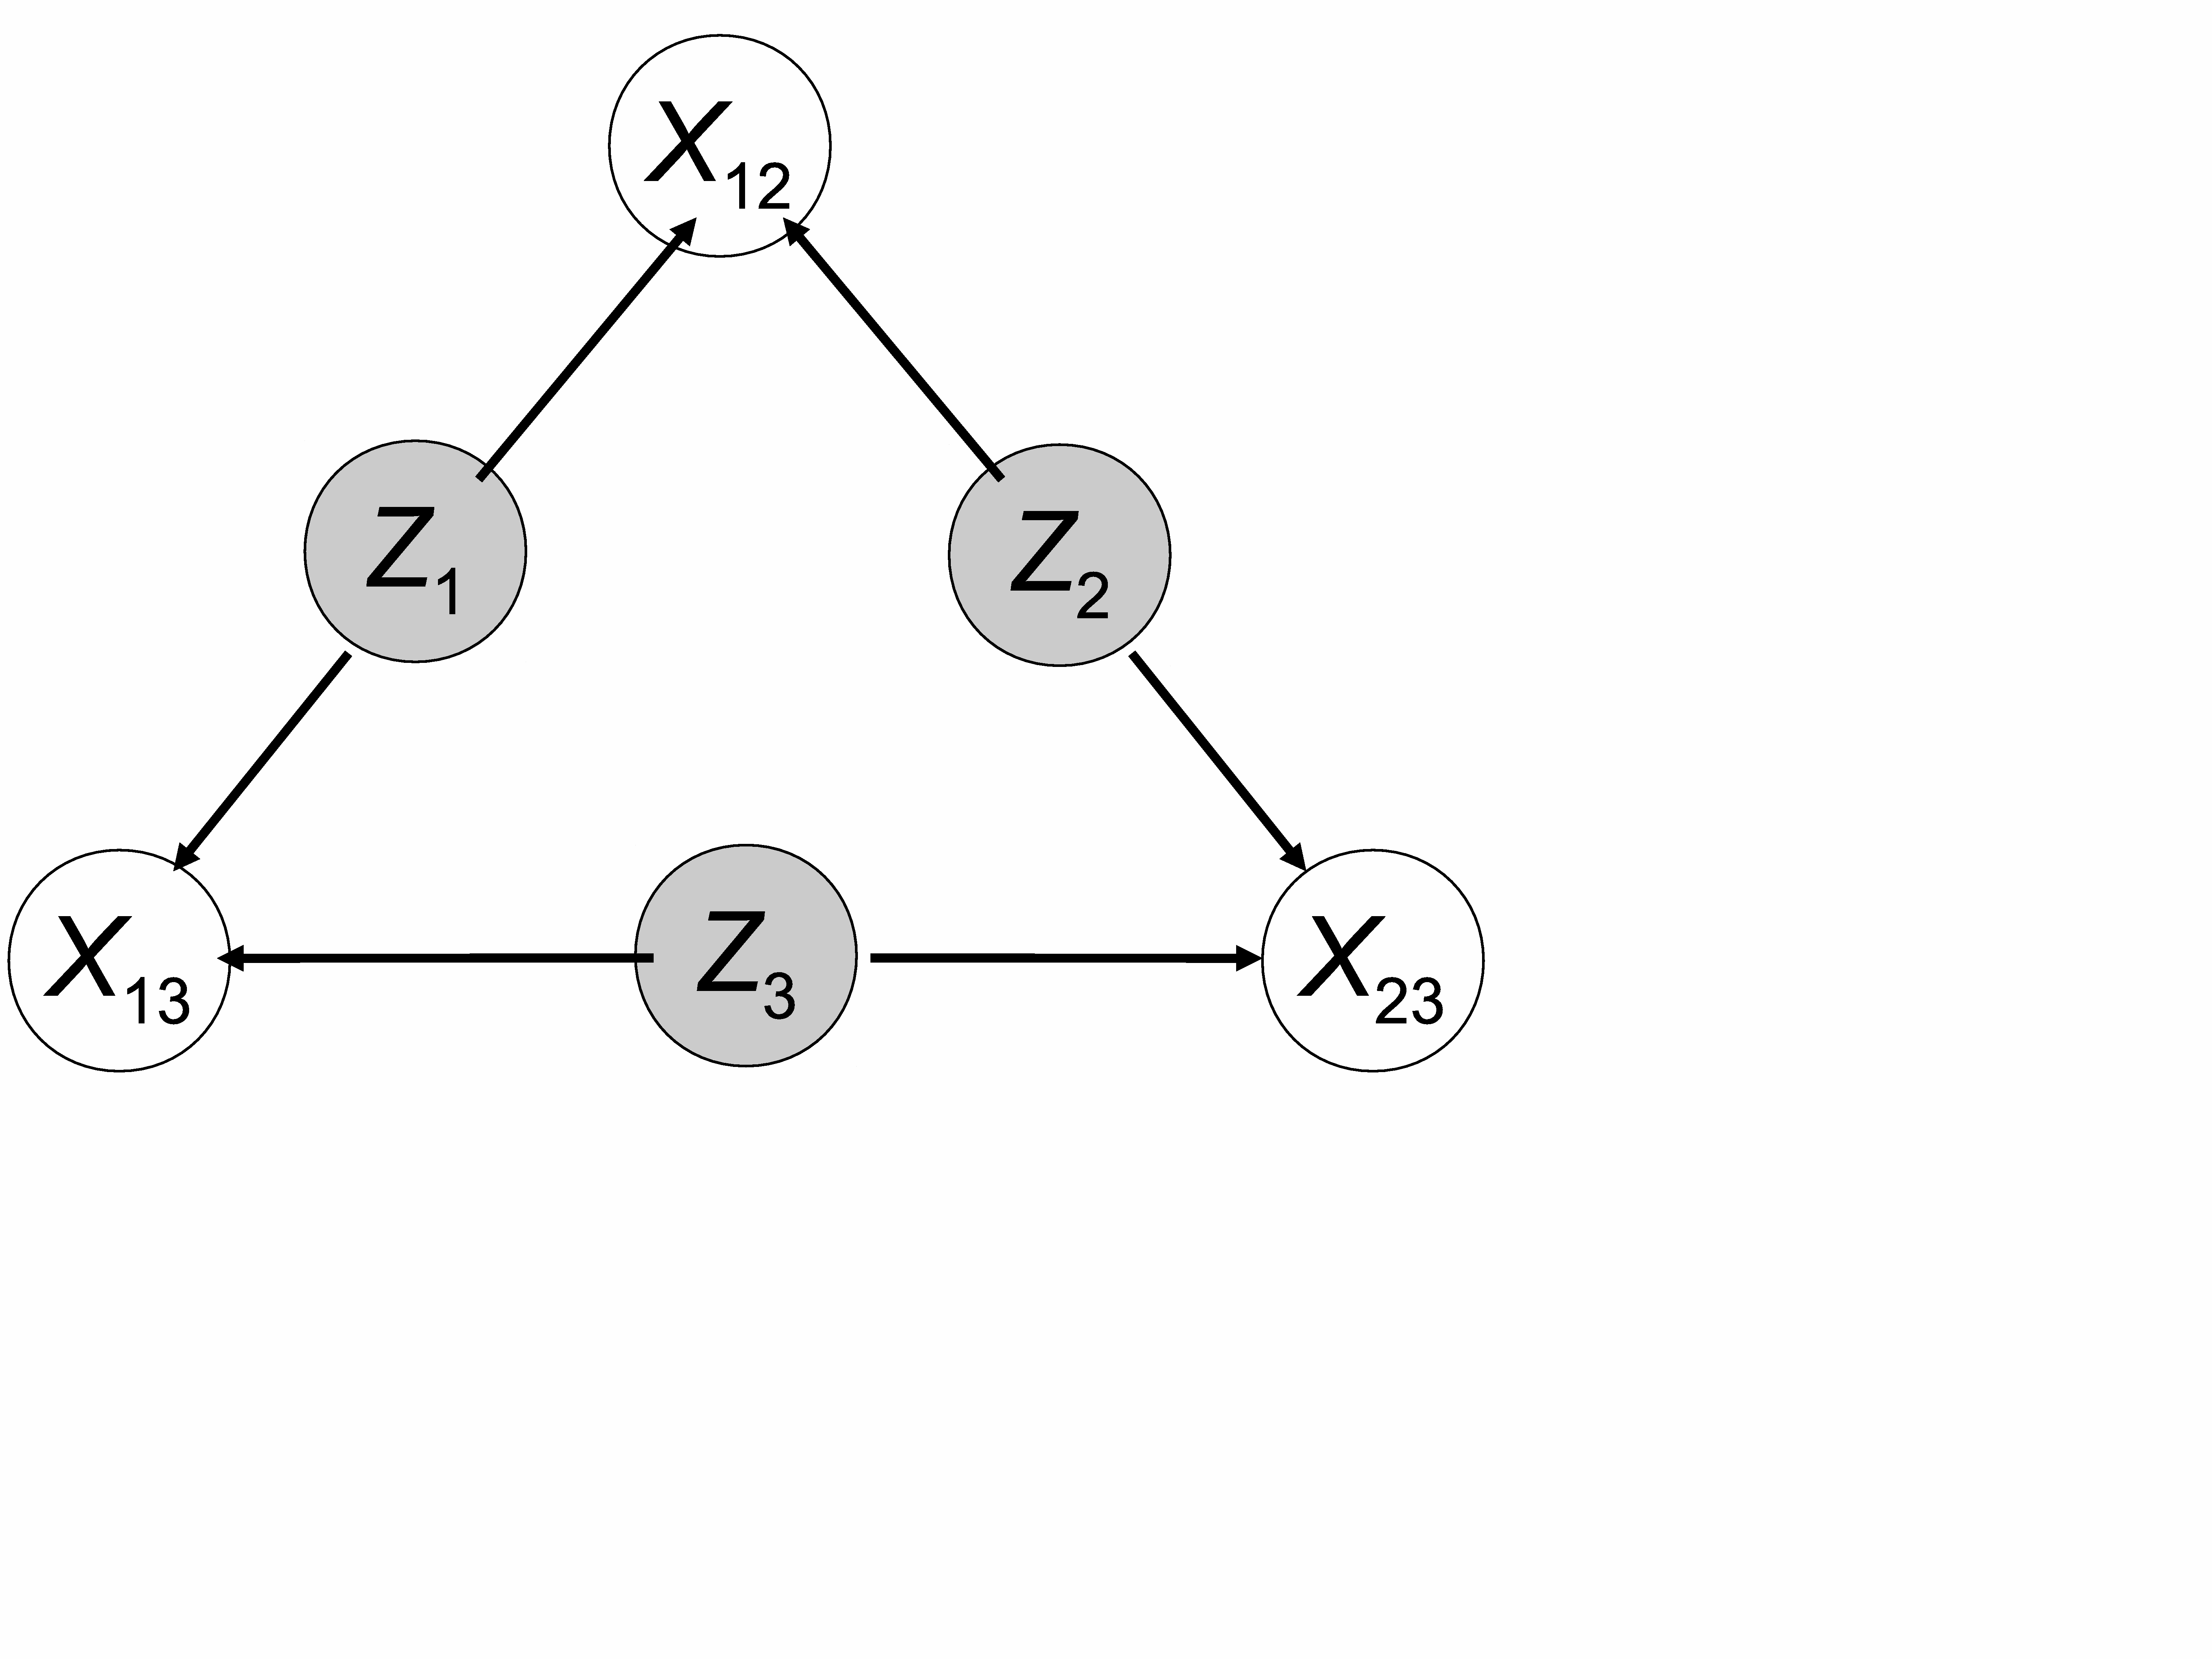
\includegraphics[width=.7\textwidth, clip=]{../FIGURES/FigSBM-Z-X}
        \onslide<3>
        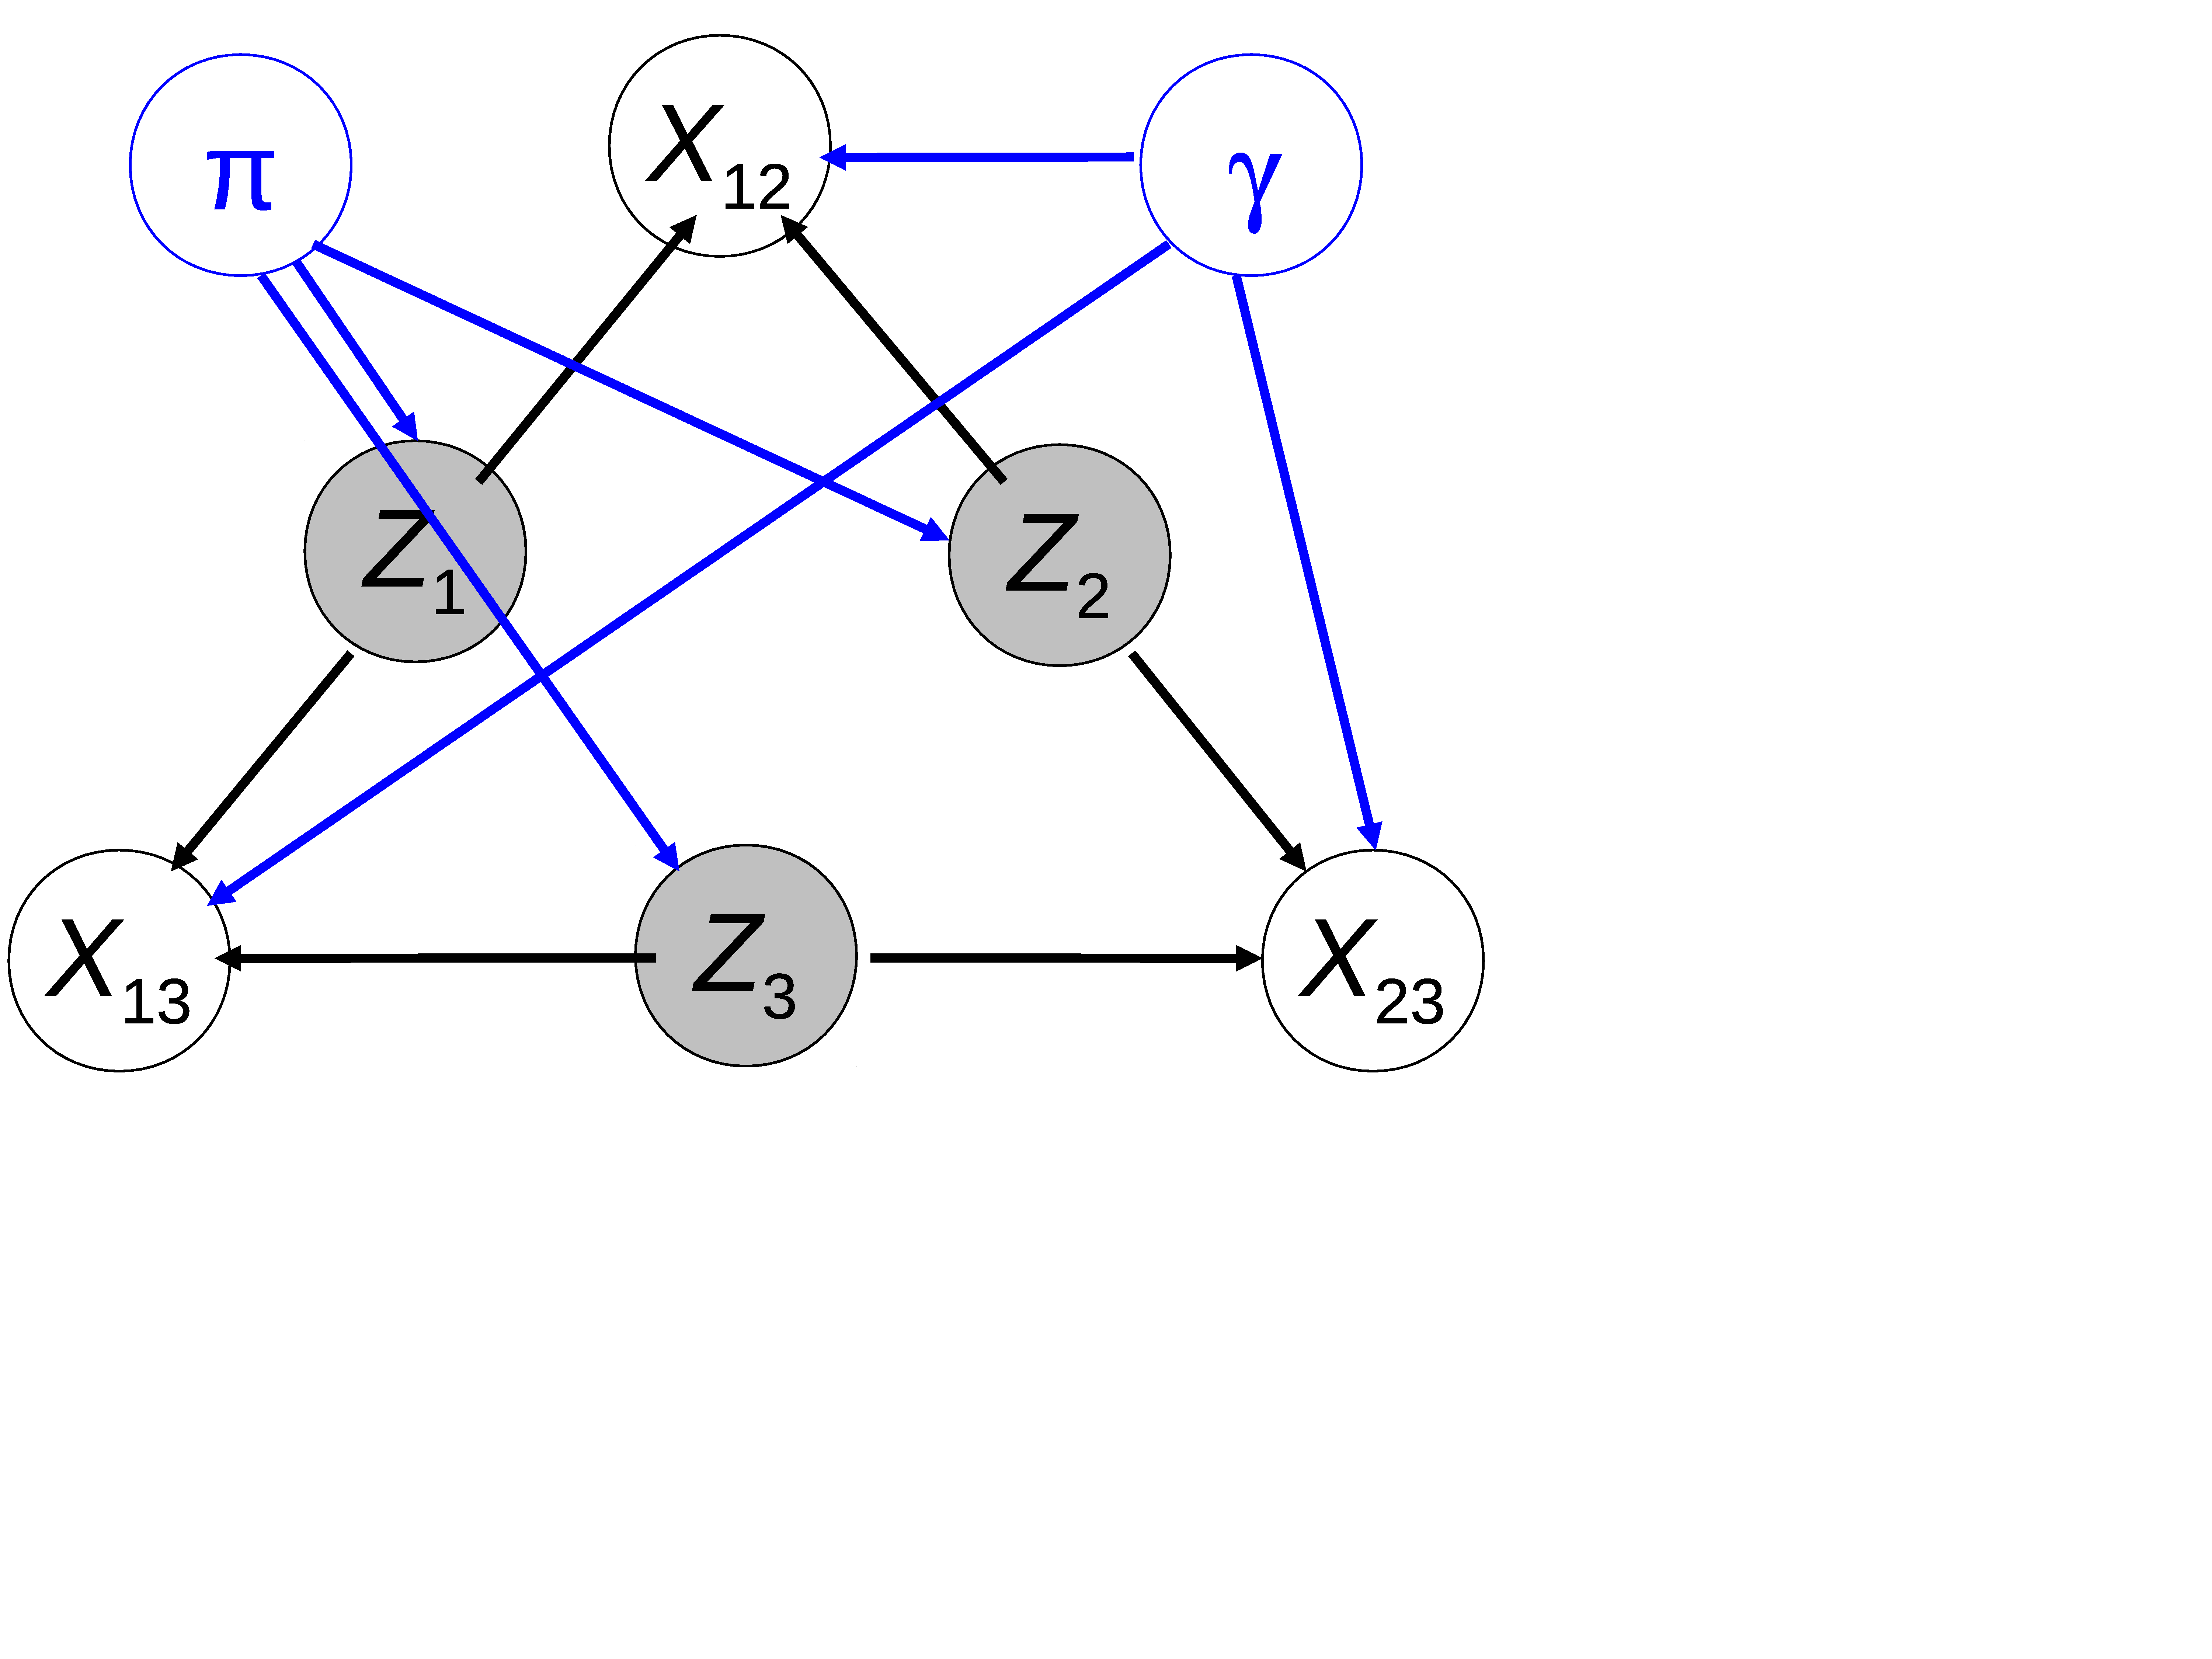
\includegraphics[width=.7\textwidth, clip=]{../FIGURES/FigSBM-Bayes-1}
        \onslide<4>
        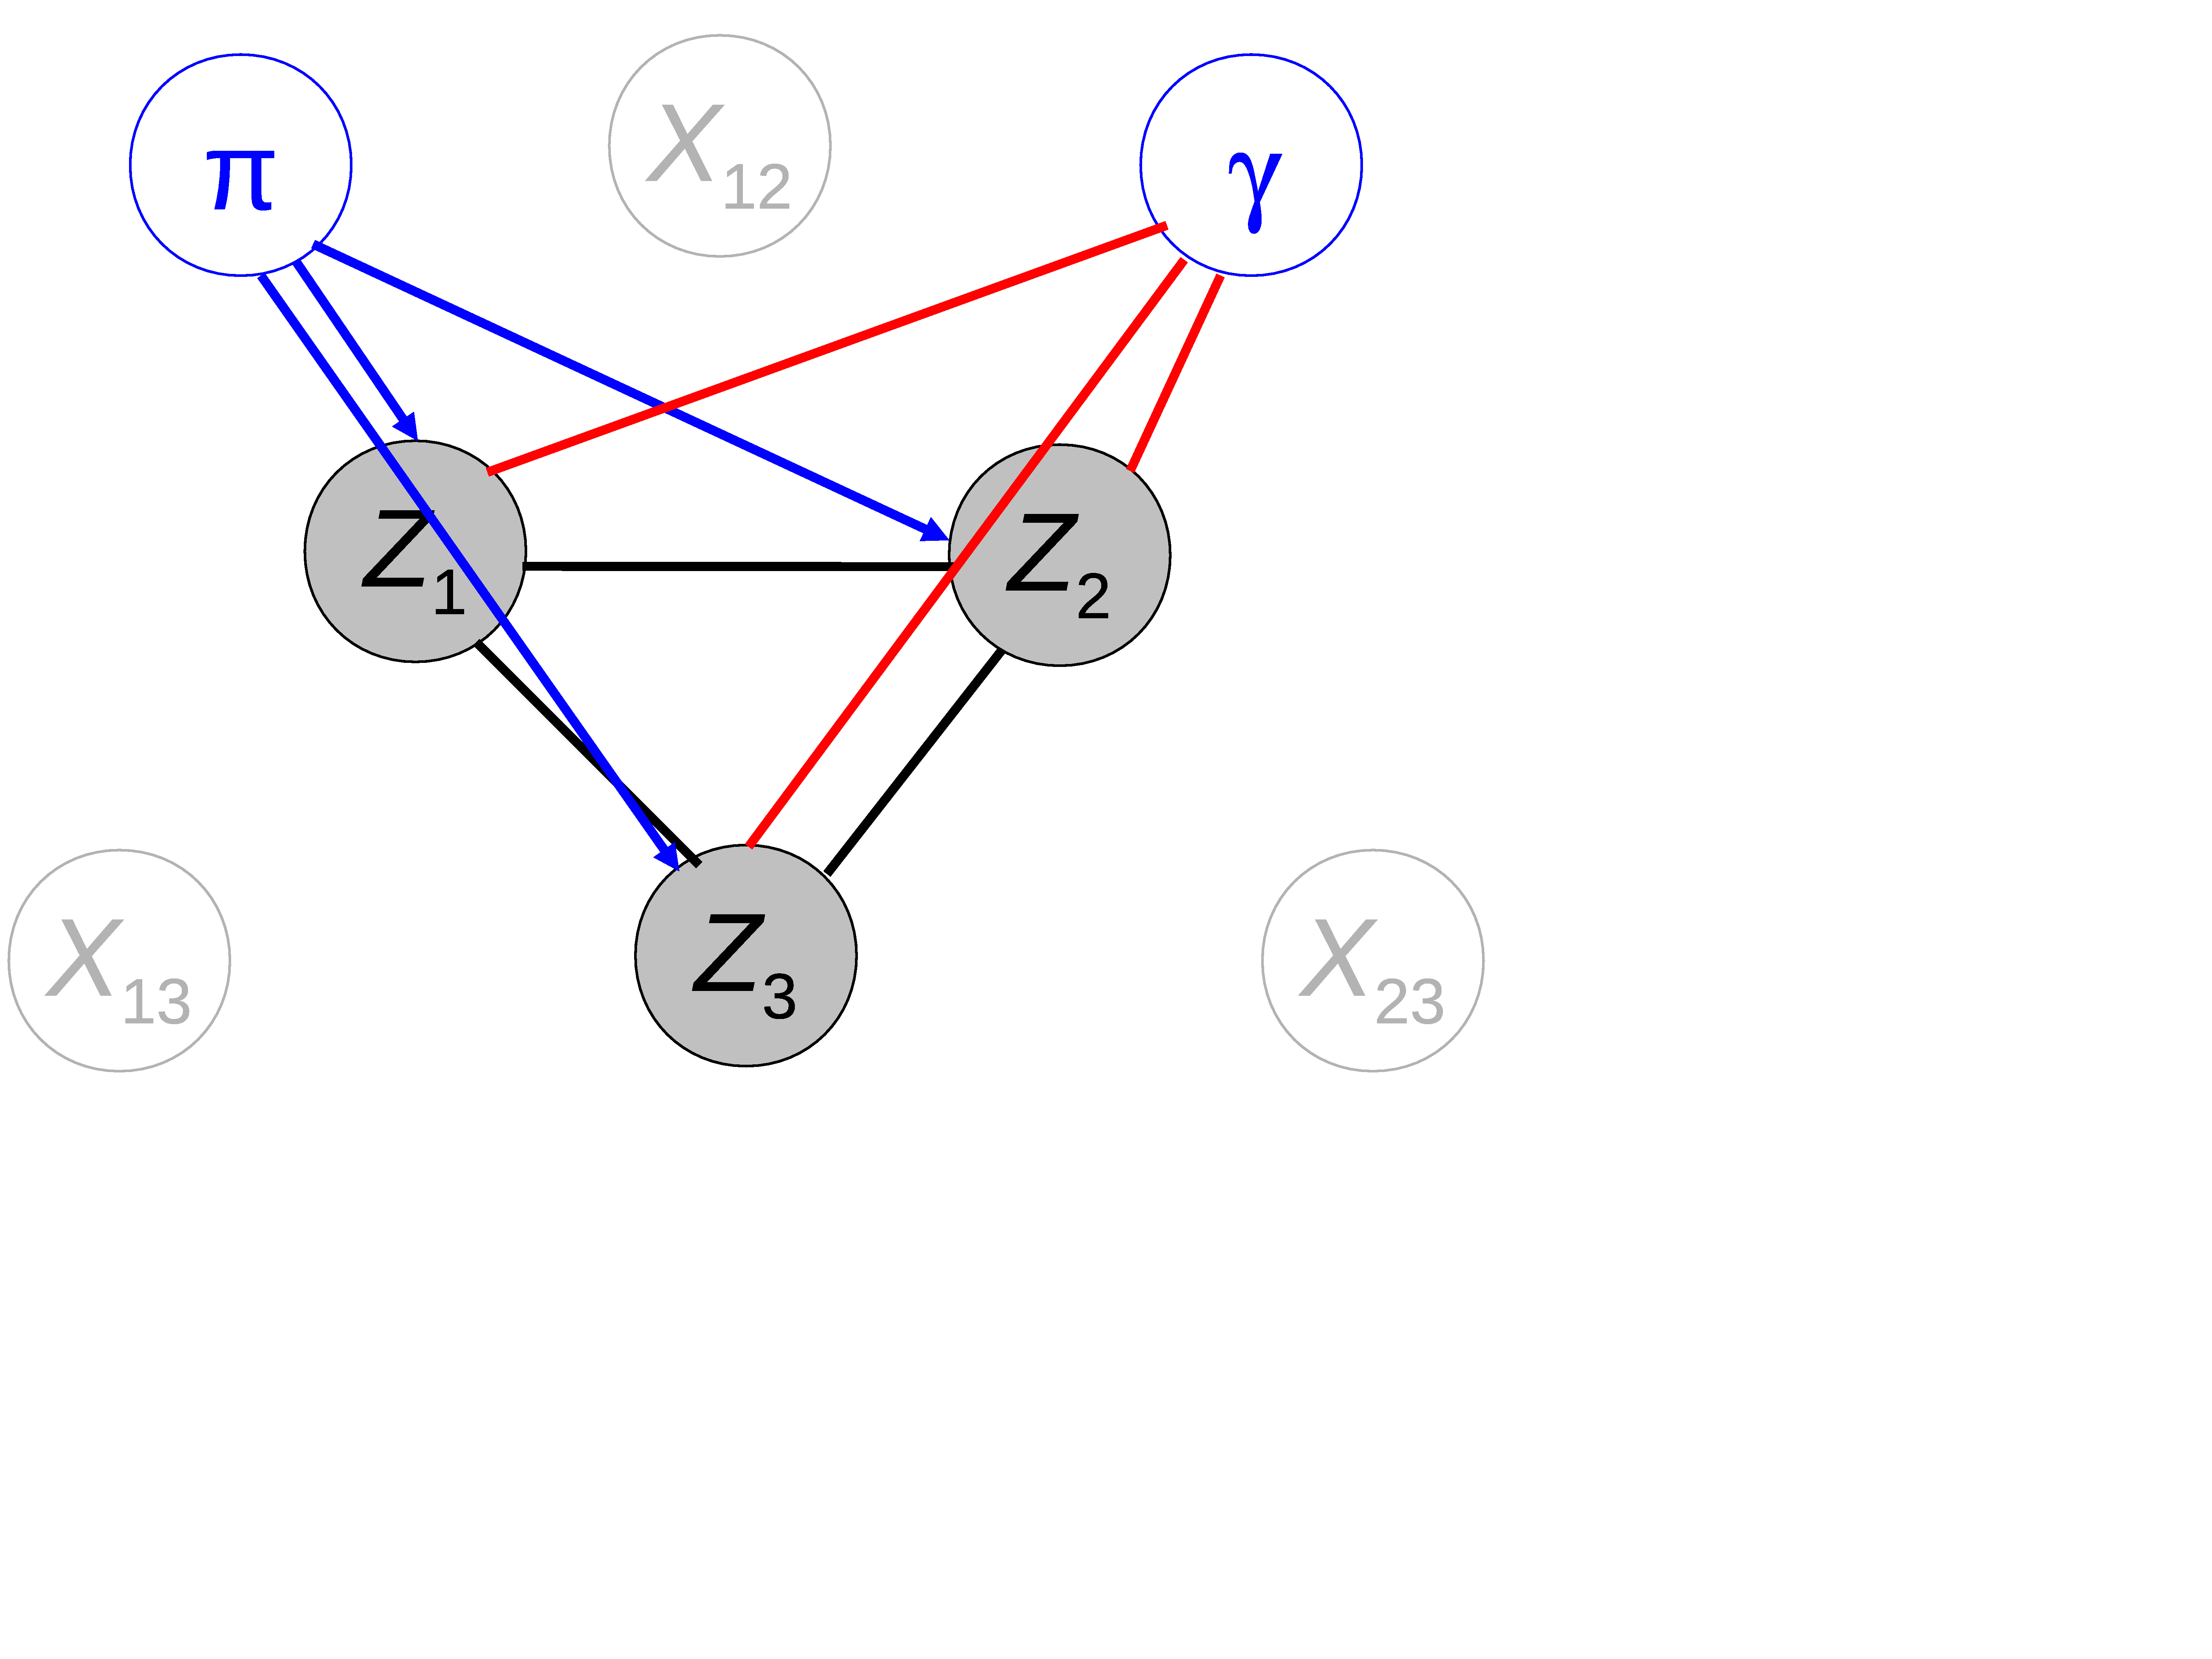
\includegraphics[width=.7\textwidth, clip=]{../FIGURES/FigSBM-Bayes-2}
      \end{overprint}
    \end{tabular}
  \end{tabular}
  
%   \onslide+<4>{
%     \vspace{-1cm}
%     Variational techniques can provide an approximation
%     $$
%     Q(Z, \theta) \simeq P(Z, \theta | X).
%     $$}
  }

%====================================================================
\frame{\frametitle{Variational approximation}

  Allows to compute optimal\footnote{here we mean in terms of K�llback-Leibler divergence} approximate distributions.
  
  \begin{itemize}
   \item \paragraph{Variational EM:}
   $$
   P_\theta(Z|X) \approx Q(Z) := \prod_i Q_i(Z_i) 
   $$
   Usefull and asymptotically exact for SBM  \refer{DPR08,CDP11,MaM13}. \\ ~
   \item \pause \paragraph{Variational Bayes EM:}
   $$
   P(Z, \theta | X) \approx Q(Z, \theta) := \prod_i Q_i(Z_i) \times Q_{\theta}(\theta) 
   $$
   in the exponential family / conjugate prior context \refer{BeG03}. \\
   Theoretical arguments and empirical evidence of its good behavior for SBM \refer{LBA11b,GDR11}.
  \end{itemize}

}

%====================================================================
\frame{ \frametitle{Why does it work for SBM ?}

  \vspace{-.05\textheight}
  \begin{tabular}{cc}
   \begin{tabular}{p{.4\textwidth}}
   Degree distribution = mixture of binomials. \\
   \bigskip 
   Binomials concentrate very fast toward their respective means. \\
   \bigskip 
   The classification problem is asymptotically 'trivial'. \\
   \bigskip
   Efficient alternatives to VEM exist for large networks \refer{CDR12}.
   \end{tabular}
   &
  \hspace{-.1\textheight}
  \begin{tabular}{c}
  \vspace{-.12\textheight}
  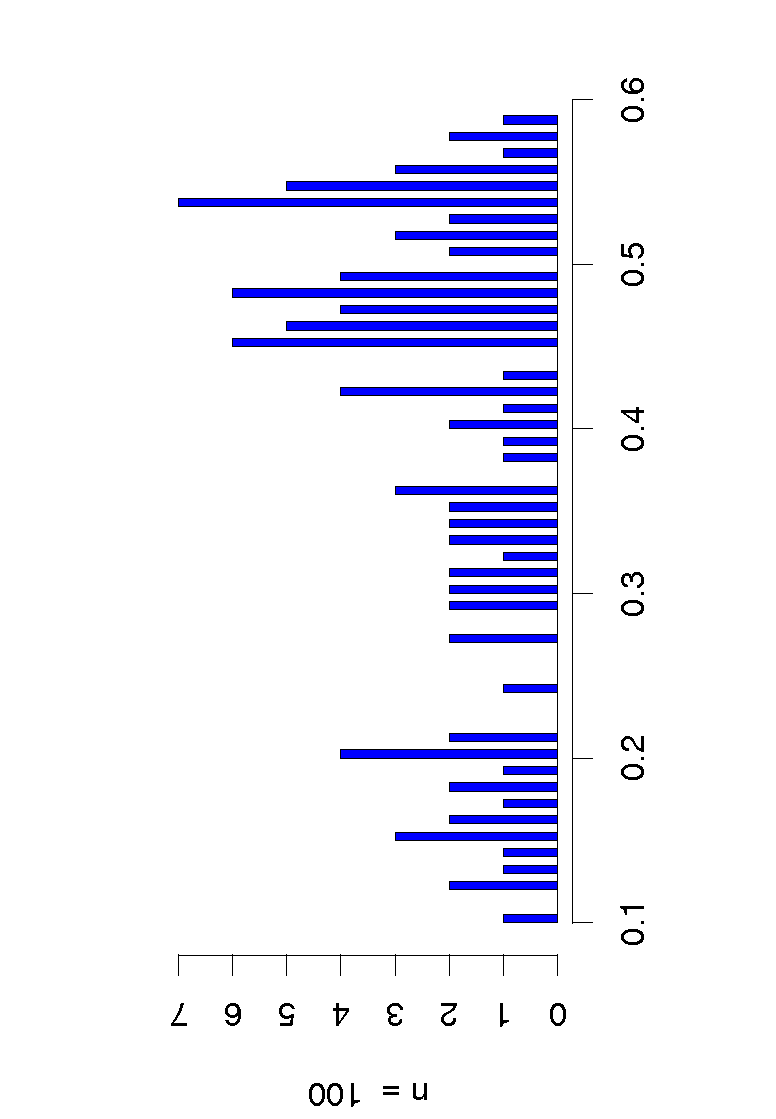
\includegraphics[width=.27\textwidth, height=.8\textheight, angle=270]{../FIGURES/ConcentrBinom-n100} \\
  \vspace{-.12\textheight}
  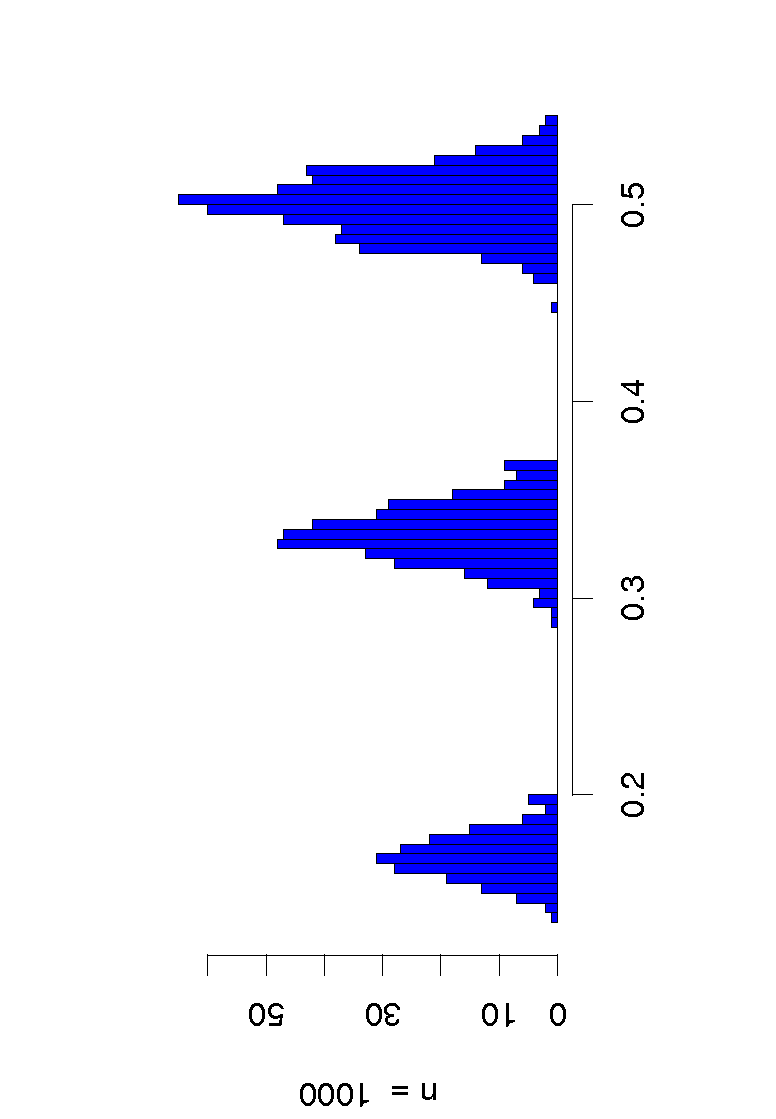
\includegraphics[width=.27\textwidth, height=.8\textheight, angle=270]{../FIGURES/ConcentrBinom-n1000} \\
  \vspace{-.12\textheight}
  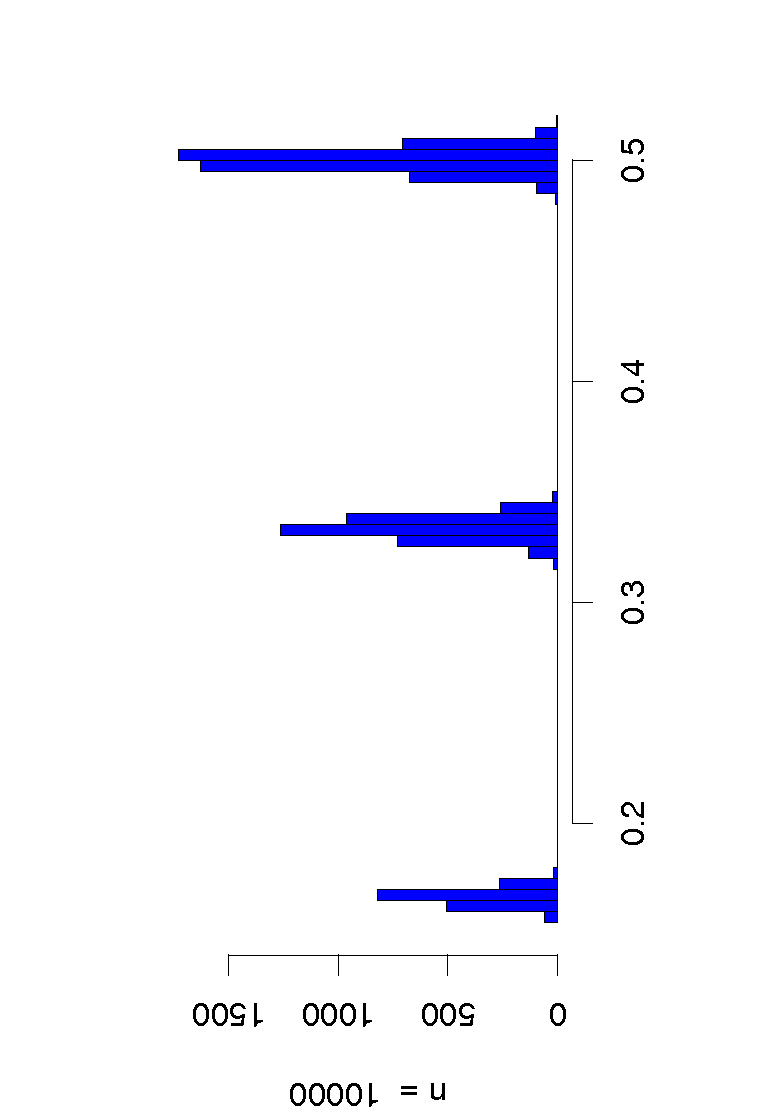
\includegraphics[width=.27\textwidth, height=.8\textheight, angle=270]{../FIGURES/ConcentrBinom-n10000} \\
  ~ \\ ~ 
   \end{tabular}
  \end{tabular}

}

%====================================================================
\frame{\frametitle{Bayesian model averaging}

%   There is no 'true' $K$ when inferring the graphon of a $W$ graph.
  
%   \bigskip
  \paragraph{Bayesian model averaging (BMA).} Consider a series of models $1, \dots, K, \dots$ in which a certain function of the parameter $f(\theta)$ can always be defined.
  
  \bigskip
  \begin{itemize}
   \item \pause Bayesian inference within each model $K$ provides the posterior
   $$
   P(\theta|K, X) \qquad \rightarrow \qquad P(f(\theta) | K, X).
   $$ ~\\
   \item \pause BMA \refer{HMR99} relies on the marginal posterior of $f(\theta)$:
   $$
   P(f(\theta) | X) = \sum_K P(K | X) P(f(\theta) | K, X).
   $$
  \end{itemize}

}

%====================================================================
\frame{\frametitle{Variational Bayes model averaging}

  \paragraph{Pushing it further:} Consider the model $K$ as an additional hidden variable:
  \begin{eqnarray*}
  P(Z, \theta, K|X) & \approx & Q(Z, \theta, K) \\
  & := & Q_{Z|K}(Z|K) \times Q_{\theta|K}(\theta|K) \times Q_{K}(K)  \end{eqnarray*}
  Note that no additional independence assumption is needed.
  
  \bigskip \bigskip \pause
  \paragraph{Variational Bayes model averaging (VBMA).} The optimal\footnote{in terms of K�llback-Leibler divergence} approximation of $P(K|X)$ satisfies \refer{VMR12}: 
  $$
    Q_K^*(K) \propto P(K) e^{\log P(X|K) - KL(K)} = P(K|X) e^{-\emphase{KL(K)}}
  $$ ~ \\
  where $KL(K) = KL[Q^*(Z, \theta|K); P(Z,  \theta|X, K)]$. 

}

%====================================================================
\section{Averaging SBMs to estimate the graphon}
\frame{ \frametitle{Averaging SBMs to estimate the graphon}}
%====================================================================
\frame{ \frametitle{Inference of the graphon function} 

  \paragraph{Probabilistic point of view.}
  \begin{itemize}
   \item $W$-graph have been mostly studied in the probability literature as a limit for dense graphs: \refer{LoS06}, \refer{DiJ08}
   \item Intrinsic un-identifiability of the graphon function $\gamma$ is often overcome by imposing that $u \mapsto \int \gamma(u, v) \dd v$ is monotonous increasing.
   \item Motif (sub-graph) frequencies are invariant characteristics of a $W$-graph.
  \end{itemize}

  \bigskip \bigskip \pause
  \paragraph{Statistical point of view.}
  \begin{itemize}
   \item Not much attention has been paid to its inference until very recently: \refer{Cha12}, \refer{ACC13}, \refer{WoO13}, ...
   \item The two latter also uses SBM as a proxy for $W$-graph.
  \end{itemize}
}

%====================================================================
\frame{ \frametitle{SBM as a $W$-graph model}

  \begin{tabular}{cc}
    \hspace{-.5cm}
    \begin{tabular}{p{.5\textwidth}}
	 Latent variables:
	 $$
	 (Z_i) \text{ iid } \sim \Mcal(1, \pi)
	 $$ ~\\
	 Blockwise constant graphon:
	 $$
	 \gamma(z, z') = \gamma_{k\ell}
	 $$ ~\\
	 Edges:
	 $$
	 \Pr\{X_{ij} = 1\} = \gamma(Z_i, Z_j)
	 $$    
	 \end{tabular}
    & 
    \hspace{-.1\textwidth}
    \begin{tabular}{p{.5\textwidth}}
	 Graphon function $\gamma^{SBM}_K(z, z')$ \\
      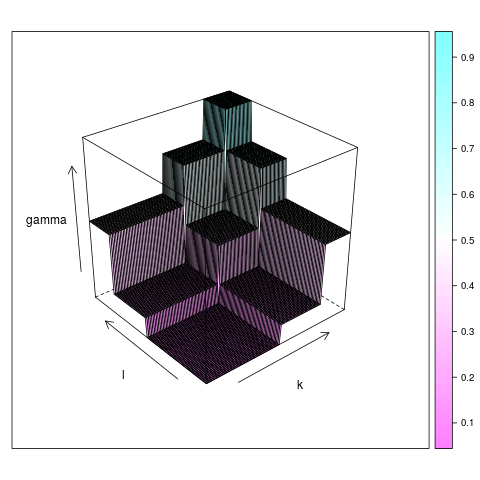
\includegraphics[width=.5\textwidth]{../FIGURES/FigCLADAG-SBM-graphon} \\
    \end{tabular}
  \end{tabular}

  \ra block widths $= \pi_k$, block heights $\gamma_{k\ell}$
 }

%====================================================================
\frame{ \frametitle{Variational Bayes estimation of $\gamma(z, z')$}

%   \paragraph{General idea.} Estimate the true $\gamma$ with a blockwise constant function $\gamma_K^{SBM}$ with $K$ classes.

  \begin{tabular}{cc}
    \hspace{-.5cm}
    \begin{tabular}{p{.5\textwidth}}
    \paragraph{VBEM inference} provides the \\approximate posteriors:
    \begin{eqnarray*}
    (\pi | X) & \approx & \text{Dir}(\pi^*) \\
    (\gamma_{k\ell} | X) & \approx & \text{Beta}(\gamma^{0*}_{k\ell}, \gamma^{1*}_{k\ell}) 
    \end{eqnarray*}
    ~
    
    \paragraph{Estimate of $\gamma(u, v)$.} 
    Due \\
    to the uncertainty of the $\pi_k$, \\
    the posterior mean of $\gamma^{SBM}_K$  \\
    is smooth
    
    \bigskip \bigskip 
    (Explicit integration using \refer{GoS10})
%     $$
%     \widehat{\gamma}_K^{SBM}(u, v) = \widetilde{\Esp}\left(\gamma_{C(u), C(v)} | X\right)
%     $$
%     where $C(u) = 1 + \sum_k \Ibb\{\sigma_k \leq u\}$. \\ ~
%     \\
%     \refer{GoS10}
    \end{tabular}
    & 
    \hspace{-.1\textwidth}
    \begin{tabular}{p{.5\textwidth}}
	 Posterior mean $\widetilde{\Esp}(\gamma^{SBM}_K(z, z') | X, K)$ \\
      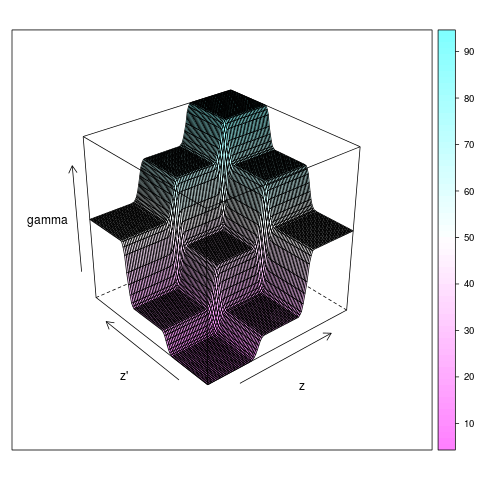
\includegraphics[width=.5\textwidth]{../FIGURES/FigGraphon-SBM-average} \\
% 	 Posterior mean of $\gamma^{SBM}_K(z, z')$ \\
%     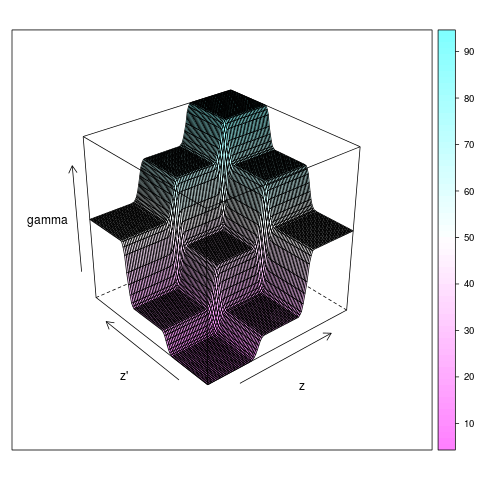
\includegraphics[width=.6\textwidth]{../FIGURES/FigGraphon-SBM-average} \\
    \end{tabular}
  \end{tabular}
  
}

%====================================================================
\frame{ \frametitle{Averaging SBMs}

  \paragraph{Model averaging:} There is no 'true $K$' in the $W$-graph model.

  \bigskip \bigskip
  \paragraph{Apply VBMA recipe to $\gamma(z, z')$.}
  For $K = 1 .. K_{\max}$, fit an SBM model via VBEM and compute
  $$
  \widehat{\gamma}_K^{SBM}(z, z') = \widetilde{\Esp}[\gamma_{C(z), C(z')} | X, K].
  $$
  
  \pause \bigskip \bigskip
  Then perform model averaging as
  $$
  \widehat{\gamma}(z, z') = \widetilde{\Esp}[\gamma_{C(z), C(z')} | X] = \sum_K Q^*_K(K) \widehat{\gamma}_K^{SBM}(z, z').
  $$
%   \end{itemize}

}

%====================================================================
\frame{ \frametitle{Some simulations}

  \begin{tabular}{cc}
    \hspace{-.5cm}
    \begin{tabular}{p{.5\textwidth}}
    \paragraph{Design.} Symetric graphon:
    $$
    \gamma(u, v) = \rho \lambda^2 (uv)^{\lambda-1}
    $$
    \begin{itemize}
     \item $\lambda \uparrow$: imbalanced graph 
     \item $\rho \uparrow$: dense graph
    \end{itemize}
    
    \bigskip
    \paragraph{Results.}
    \begin{itemize}
     \item More complex models as $n$ and $\lambda$ $\uparrow$
     \item Posterior fairly concentrated
    \end{itemize}

    \end{tabular}
    & 
    \hspace{-.1\textwidth}
    \begin{tabular}{p{.5\textwidth}}
    Variational posterior for $K$: $Q^*(K)$.
    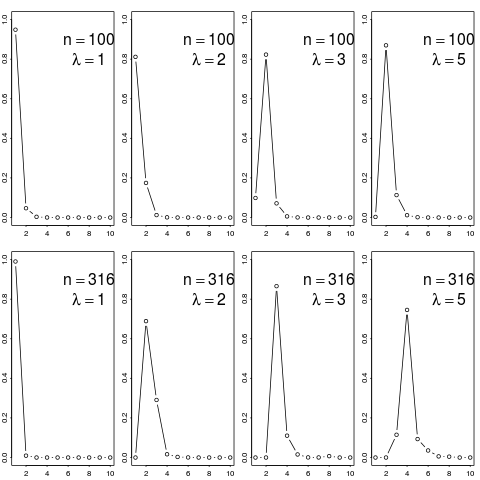
\includegraphics[width=.5\textwidth]{../FIGURES/PostDistQ-Talk-Lambda-N-rho0316227766016838}
    \end{tabular}
  \end{tabular}

}

%====================================================================
\section{French political blogosphere}
\frame{ \frametitle{French political blogosphere}}
%====================================================================
\frame{ \frametitle{French political blogosphere} 

  \paragraph{Website network.} French political blogs: 196 nodes, 1432 edges.
  $$
  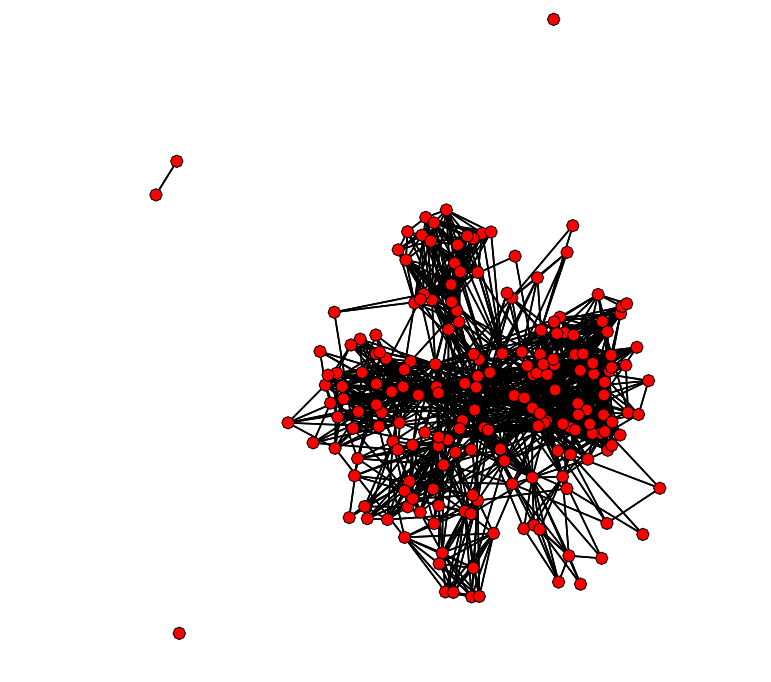
\includegraphics[width=.65\textwidth]{../FIGURES/Blogosphere-raw}
  $$
}

%====================================================================
\frame{ \frametitle{French political blogosphere}

  \paragraph{Infered graphon.} $\widehat{W}(u, v) = \widetilde{\Esp}(\gamma(u, v)|X)$
  \begin{overprint}
  \onslide<1>
  $$
  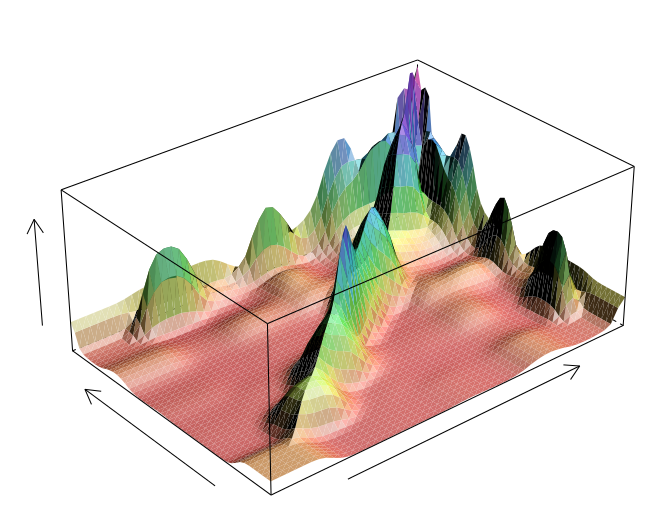
\includegraphics[width=.65\textwidth]{../FIGURES/Blogosphere-graphon}
  $$
  \onslide<2>
  \vspace{-.05\textheight}
  $$
  \includegraphics[width=.6\textwidth]{../FIGURES/Blogosphere-contour}
  $$
  \end{overprint}
}


%====================================================================
\frame{ \frametitle{Network motifs}

  \vspace{-0.1\textheight}
  $$
  \begin{tabular}{cccccc}
  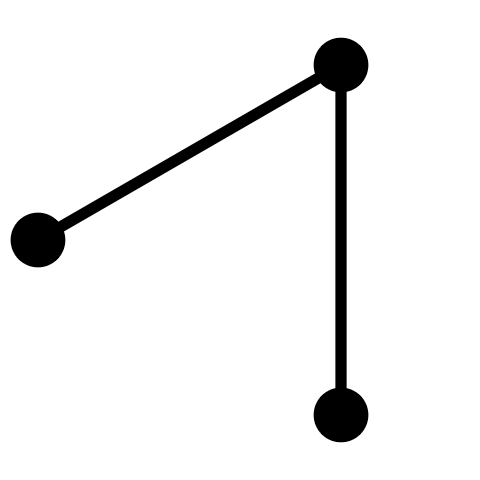
\includegraphics[width=.1\textwidth]{../FIGURES/FigMotif-V}
  & 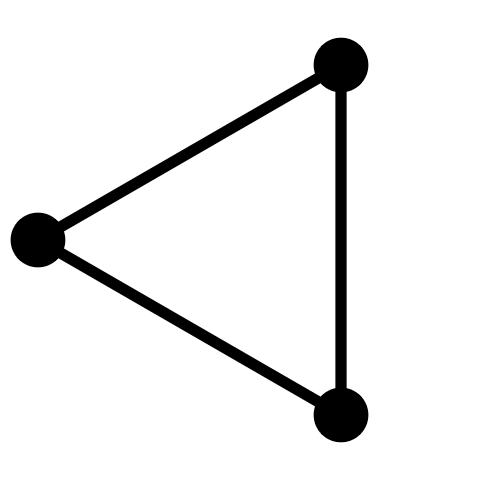
\includegraphics[width=.1\textwidth]{../FIGURES/FigMotif-Triangle}
  & 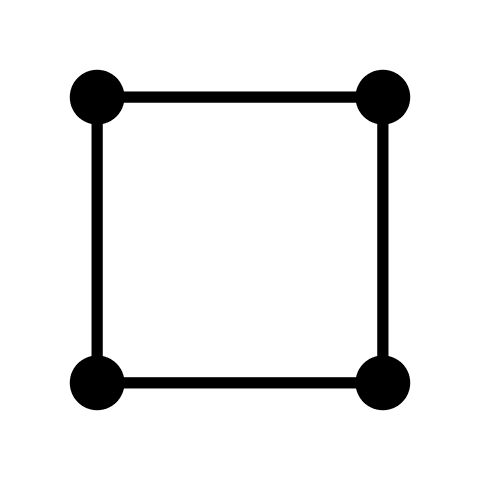
\includegraphics[width=.1\textwidth]{../FIGURES/FigMotif-Square}
  & 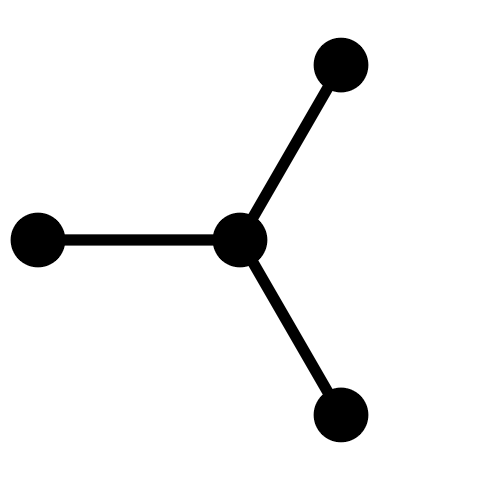
\includegraphics[width=.1\textwidth]{../FIGURES/FigMotif-Star3}
  & 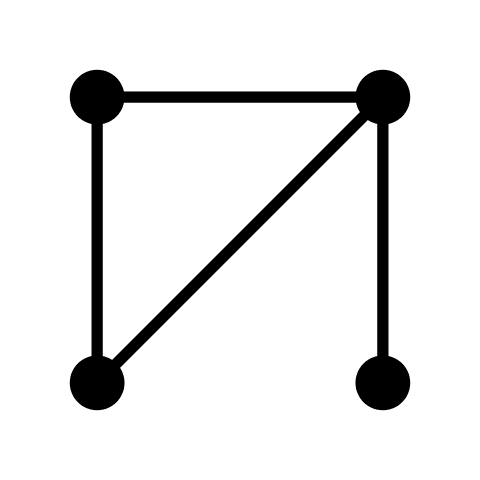
\includegraphics[width=.1\textwidth]{../FIGURES/FigMotif-Whisker}
  & 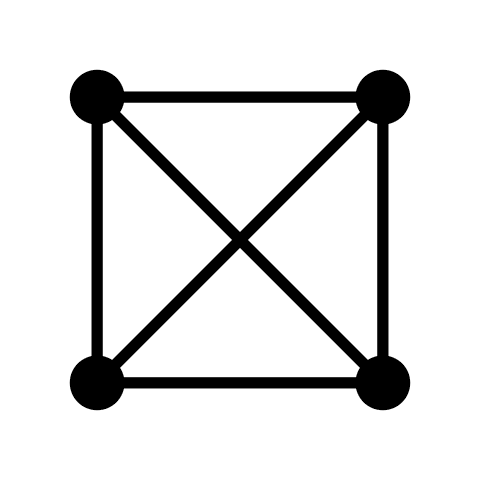
\includegraphics[width=.1\textwidth]{../FIGURES/FigMotif-Clique4}
  \end{tabular}
  $$
  
  \begin{itemize}
  \item Network motifs have sociological interpretation (e.g. triangles).
  \item The first moments $\Esp N(m), \Var N (m)$ of the count are known under SBM \refer{PDK08}: 
   $$
   \Esp_{SBM} N(m) \propto  \mu_{SBM}(m) = f(\theta_{SBM}) %, \Var_{SBM(K)} N(m)
   $$
   \item Motif probability can be estimated as 
   $$
   \widehat{\mu}(m) = \sum_k Q_K^*(K) \widetilde{\Esp}(\mu_{SBM}(m) | X, K)
   $$
  \end{itemize}
  \ra Goodness of fit criterion
   
}

%====================================================================
\frame{ \frametitle{Network motifs in the blogosphere}

\vspace{-0.1\textheight}
$$
\begin{tabular}{crrrrr}
  \hline
 Motif & Count & Mean & Std. dev. & approx \\ 
 & ($\times 10^3$) & ($\times 10^3$) & ($\times 10^3$) & $p$-value \refer{PDK08} \\ 
%   \hline
%   1 & 29715 & 39722.11 & 8259.28 & 0.89 \\ 
%   2 & 3821 & 4512.51 & 1276.13 & 0.69 \\ 
%   3 & 608708 & 968364.08 & 336800.24 & 0.86 \\ 
%   4 & 279771 & 428867.52 & 153962.02 & 0.83 \\ 
%   5 & 47415 & 74533.94 & 35075.09 & 0.77 \\ 
%   6 & 270497 & 397053.82 & 177049.01 & 0.75 \\ 
%   7 & 62071 & 87849.83 & 47407.22 & 0.67 \\ 
%   8 & 6523 & 8818.95 & 5385.87 & 0.61 \\ 
%   \hline
  \hline
  \begin{tabular}{c} 
\includegraphics[width=.045\textwidth]{../FIGURES/FigMotif-I} \end{tabular} & 29.7 & 39.7 & 8.3 & 0.89 \\ 
  \begin{tabular}{c} 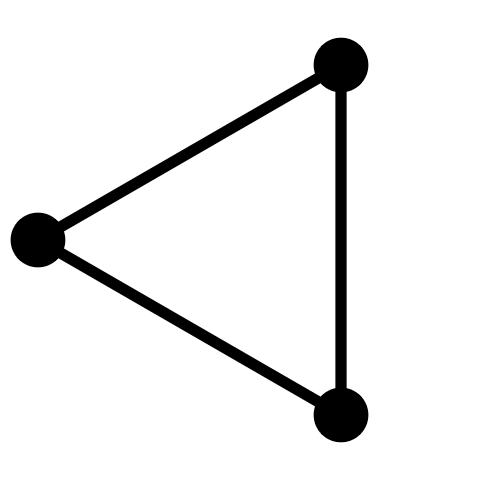
\includegraphics[width=.045\textwidth]{../FIGURES/FigMotif-Triangle} \end{tabular} & 3.8 & 4.6 & 1.3 & 0.69 \\ 
  \begin{tabular}{c} 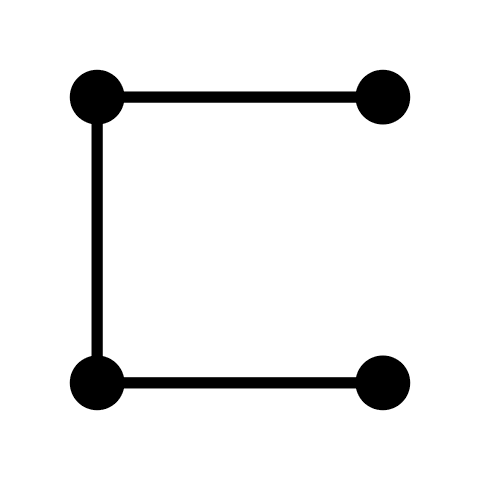
\includegraphics[width=.045\textwidth]{../FIGURES/FigMotif-Chain4} \end{tabular} & 608.7 & 968.3 & 336.8 & 0.86 \\ 
  \begin{tabular}{c} 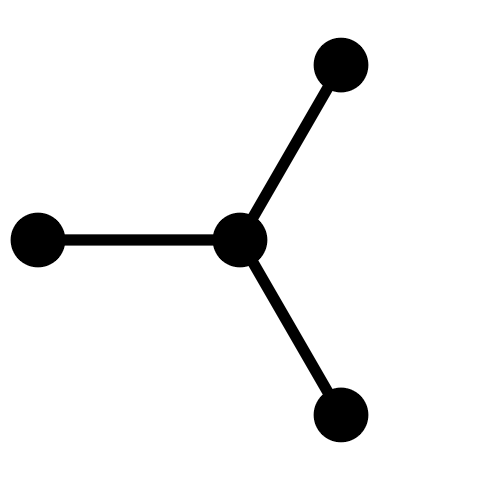
\includegraphics[width=.045\textwidth]{../FIGURES/FigMotif-Star3} \end{tabular}  & 279.8 & 428.9 & 154.0 & 0.83 \\ 
  \begin{tabular}{c} 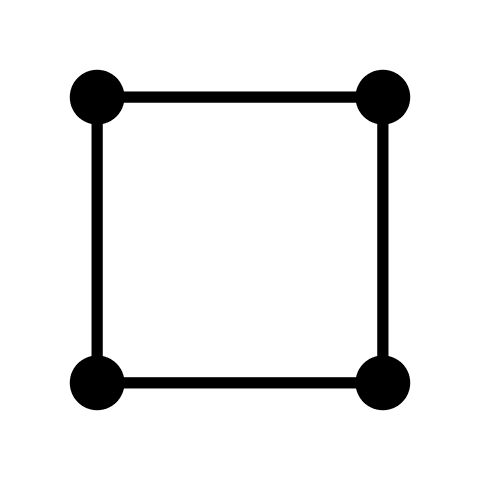
\includegraphics[width=.045\textwidth]{../FIGURES/FigMotif-Square} \end{tabular} & 47.4 & 74.5 & 35.1 & 0.77 \\ 
  \begin{tabular}{c} 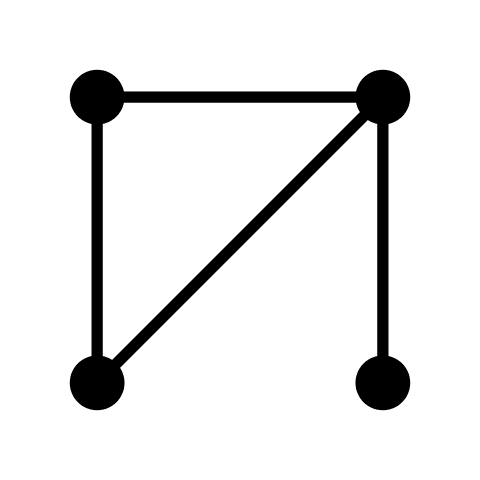
\includegraphics[width=.045\textwidth]{../FIGURES/FigMotif-Whisker} \end{tabular} & 270.5 & 397.0 & 177.0 & 0.75 \\ 
  \begin{tabular}{c} 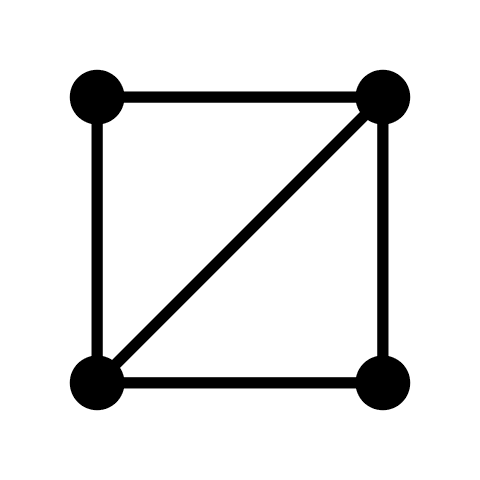
\includegraphics[width=.045\textwidth]{../FIGURES/FigMotif-SquareDiag} \end{tabular} & 62.1 & 87.8 & 47.4 & 0.67 \\ 
  \begin{tabular}{c} 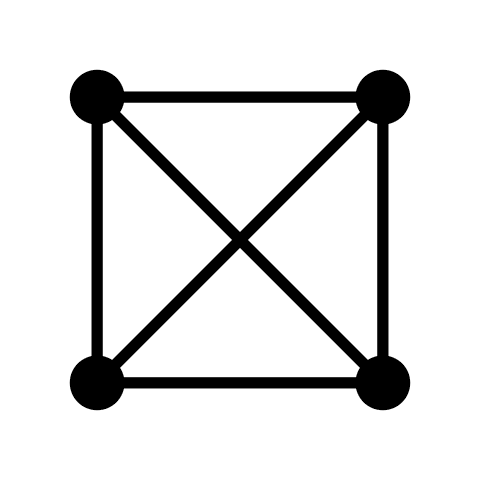
\includegraphics[width=.045\textwidth]{../FIGURES/FigMotif-Clique4} \end{tabular} & 6.5 & 8.8 & 5.4 & 0.61 \\ 
   \hline
\end{tabular}
$$

No specific structure seems to be exceptional wrt the model's expectations.

}

%====================================================================
\section{Conclusion}
%====================================================================
\frame{ \frametitle{Conclusion and future works} 

  \paragraph{Summary.}
  \begin{itemize}
   \item The graphon function of a $W$-graph is a way to summarize the global structure of a (large) network.
   \item The stochastic block model is a special case of $W$-graphs, for which many variational inference methods have been developed.
   \item Model averaging of SBM's allows the Bayesian inference of the graphon function.
   \item Motifs statistics can be used to assess the goodness of fit.
  \end{itemize}

  \bigskip \bigskip \pause 
  \paragraph{Possible extensions.}
  \begin{itemize}
  \item No formal test is available for the motif counts.
  \item The latent structure is likely to encode exogenous effects that could be encoded in covariates.
  \end{itemize}

}

%====================================================================
{\tiny
  \bibliography{/home/robin/Biblio/ARC,/home/robin/Biblio/AST,/home/robin/Biblio/SSB} 
  %\bibliographystyle{/home/robin/LATEX/Biblio/astats}
  \bibliographystyle{plain}
  }

%====================================================================
\beginbackup
%====================================================================
\frame{ \frametitle{Some more simulations}

  \begin{tabular}{cc}
%     \hspace{-.5cm}
    \begin{tabular}{cc}
    $RMSE[\gamma(z, z')]$ & $KL[\mu(m)]$ \\
    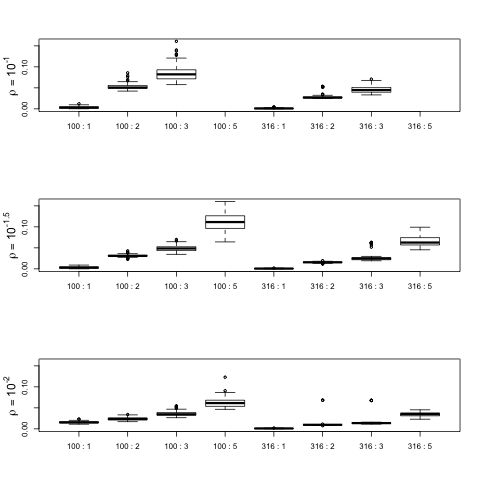
\includegraphics[width=.3\textwidth, height=.7\textheight]{../FIGURES/RMSE-rho-Nlambda} & 
    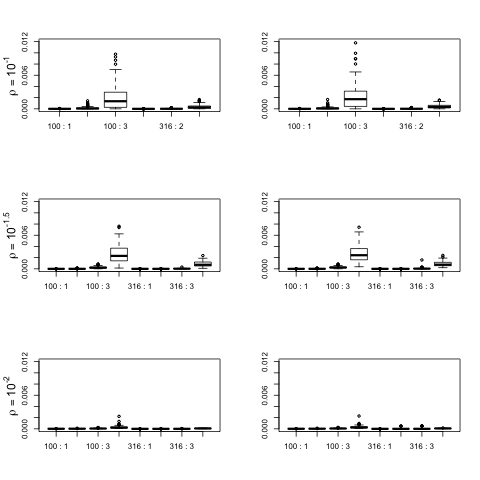
\includegraphics[width=.6\textwidth, height=.7\textheight]{../FIGURES/KL-Motif2-4-rho-Nlambda} \\
    legend: $(n : \lambda)$ & 
    \begin{tabular}{c} 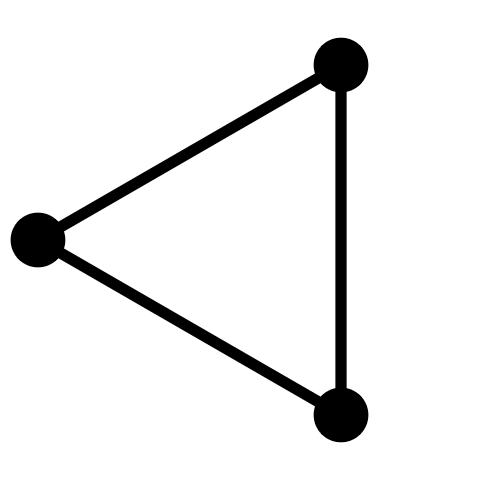
\includegraphics[width=.075\textwidth]{../FIGURES/FigMotif-Triangle} \end{tabular}
    \qquad \qquad \qquad 
    \begin{tabular}{c} 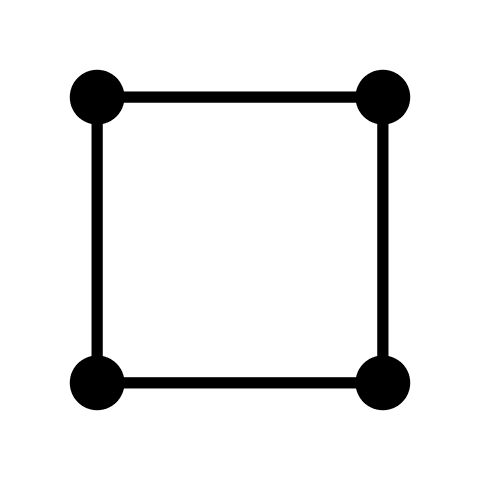
\includegraphics[width=.075\textwidth]{../FIGURES/FigMotif-Square} \end{tabular}
    \end{tabular}
  \end{tabular}

}

%====================================================================
\backupend
%====================================================================
%====================================================================
\end{document}
%====================================================================
%====================================================================

